% header
\documentclass[10pt,a4paper]{article}

\usepackage[utf8]{inputenc}
\usepackage{hyperref}
\usepackage{amssymb}
\usepackage{amsmath}
\usepackage{listings}
\usepackage{graphicx}

% the document
\begin{document}

\title{Final Solution\\
\small{Practical Lab Numerical Computing}}
\author{Andrii Lischishin \and Lars Schleithoff \and Hendrik Kleikamp}
\date{\today}
\maketitle

\section*{Worksheet 1}

\section*{Task 1}

The code generates two uniformly distributed random numbers on the interval $[0,1]$. The first random number is generated by a standard $C++$ function called $rand$.
The second random number is generated by a generator from the gsl library.
The difference lies in the generator used for creating those random numbers. The second way uses a \texttt{gsl\_rng} pointer which transports the information on the selected generator. 
One can use the same pointer for differently distributed random numbers, e.g. \texttt{double gsl\_ran\_gaussian (const gsl\_rng * r, double sigma)}, where $\mu=0$. 

If you remove the expression (double), the result will be $0$ due to rounding to the next smaller integer. The rand function creates an integer and \texttt{RAND\_MAX} is a constant integer as well. 

In fact, there won't be any different random numbers each time you run the code snippet because there is no seed declared. 

\section*{Task 2}

\begin{center}
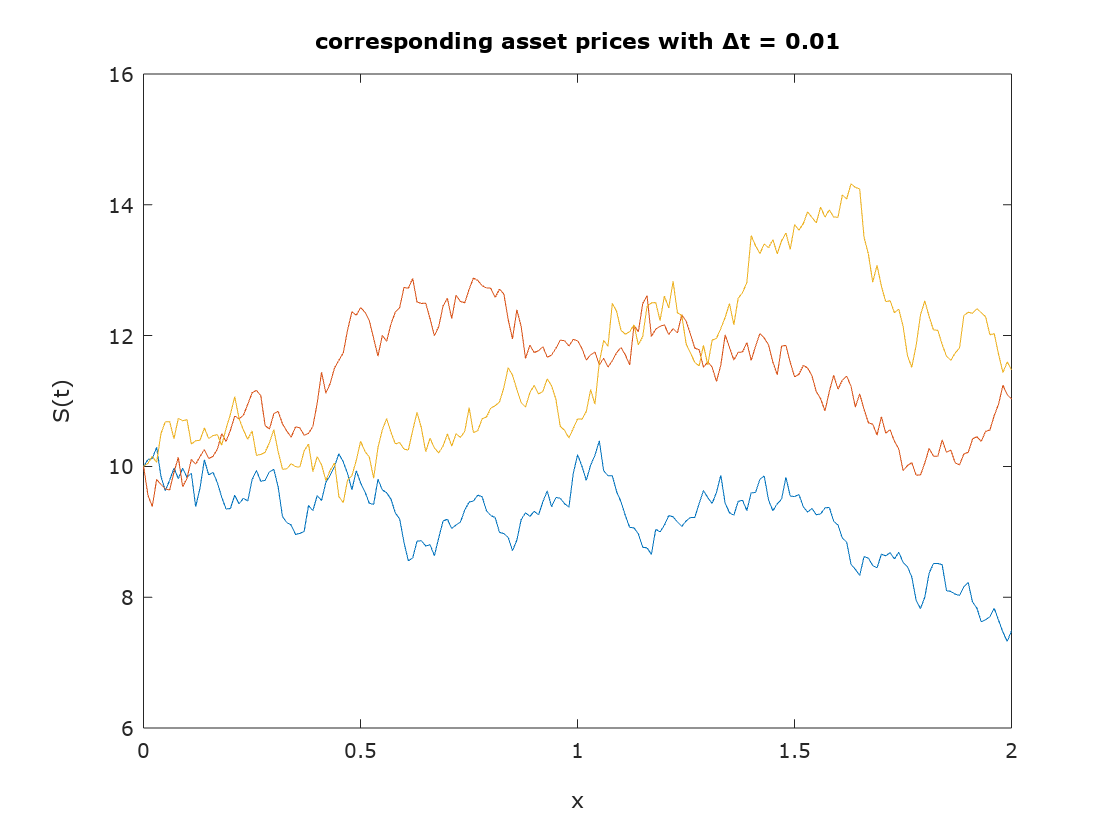
\includegraphics[scale=0.45]{asset_001.jpeg}		
\end{center}	

\begin{center}
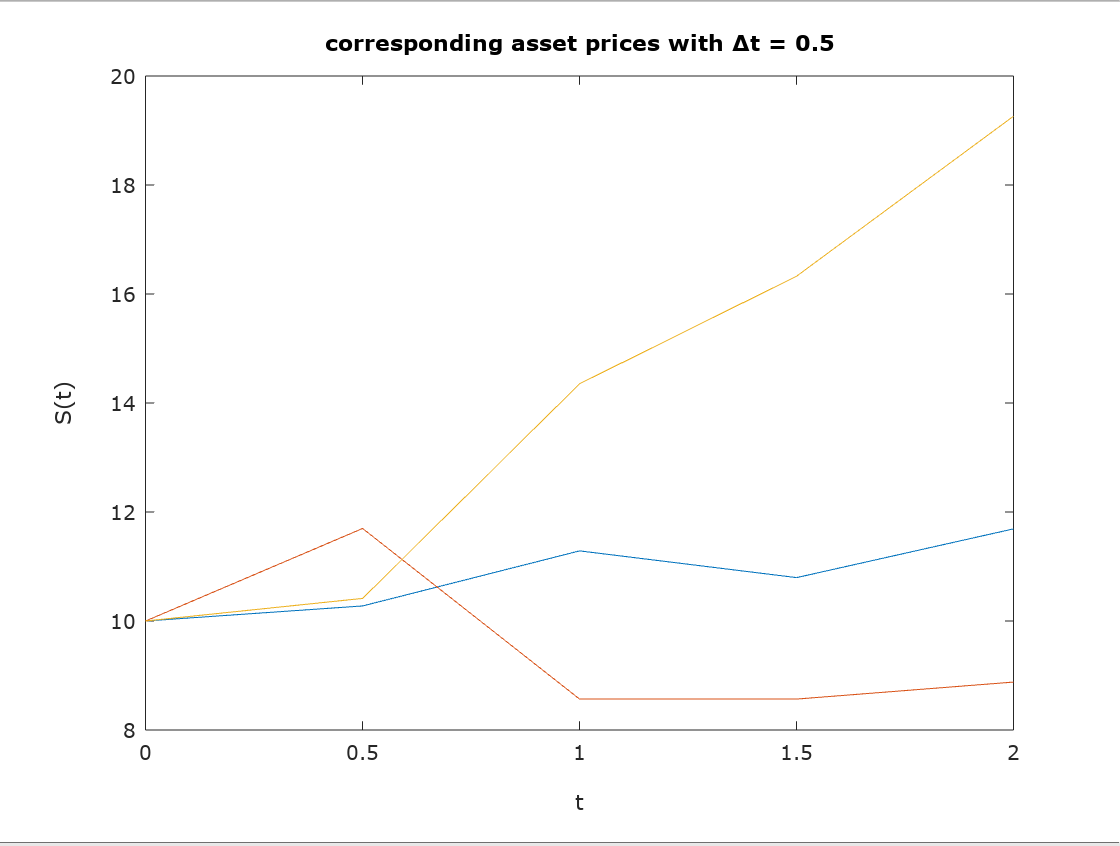
\includegraphics[scale=0.45]{asset_05.jpeg}		
\end{center}	

\section*{Task 3}

The MATLAB script divides the interval $[0,1]$ into $100$ equidistant sections. The number of random values in each interval is then depicted by the density value of the points in the plot.

Fig.1 shows what happens if the interval bounds in step $1$ of the rejection sampling algorithm are chosen to small, e.g. $[-2,2]$.  


\section*{Task 4}

Let $X$ be an uniformly distributed random variable on $(0,1)$, and $\Phi(t)=\frac{1}{\sqrt{2 \pi}}\int_{-\infty}^{t}e^{-\frac{x^2}{2}}dx$.
 
$\Phi(t)$ is continuous and monotically increasing, therefore the solution of $\Phi(t)=y$, which is $\frac{1}{\sqrt{2 \pi}}\int_{-\infty}^{t}e^{-\frac{x^2}{2}}dx=y$, is unique. Now, the inverse function $f:(0,1)\rightarrow \mathbb{R}$ takes in a value from the interval $(0,1)$ and the output is in $\mathbb{R}$.

Specifically, $\Phi(t)=\frac{1}{\sqrt{2 \pi}}\int_{a}^{b}e^{-\frac{x^2}{2}}dx=\Phi(b)-\Phi(a)$. This implies that $a\leq f(X) \leq b \Leftrightarrow \Phi(a)\leq X \leq \Phi(b)$, since $\Phi(f(X))=X$.

For this reason, applying the inverse function of the standard normal distribution to an uniformly distributed random variable leads to a standard normal distributed random variable.  

\newpage

\section*{Task 5}

The basic idea is to approximate the integral on different intervals by different functions. The first if-clause uses the symmetry of the standard normal distribution and the fact that 
\[
	\frac{1}{\sqrt{2 \pi}}\int\limits_{-\infty}^{\infty}e^{-\frac{x^2}{2}}dx=1.
\]

For $x\geq 6$, the accuracy of $8$ digits has already been reached, so the algorithm returns the value $1$.

\section*{Task 6}

\begin{center}
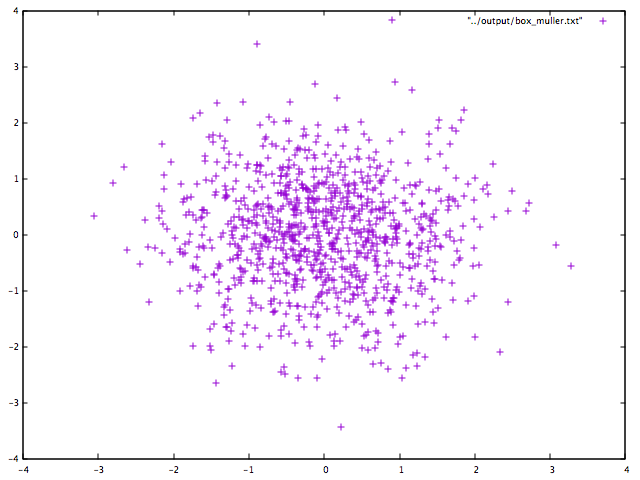
\includegraphics[scale=0.4]{box_mueller.jpeg}
\end{center}

\section*{Task 7}

By transformation to polar coordinates, it follows that
\begin{align*}
	z_1=r cos(\phi), z_2=r sin(\phi)
\end{align*}   

with $r=\sqrt{-2ln(u_1)}, \phi=2\pi u_2$. 

$\phi\in (0,2\pi)$ is uniformly distributed on circles, and the square of the radius of these circles, $r^2=Z_1^2+Z_2^2$, has Chi-squared distribution.

The product of those two random variables ist normally distributed:
\begin{align*}
\frac{1}{2}e^{-\frac{1}{2}r^2}d(r^2)d\phi = \frac{1}{2\pi}e^{-\frac{1}{2}r^2}rdrd\phi = \frac{1}{2\pi}e^{-\frac{1}{2}(z_1^2+z_2^2)}dz_1dz_2
\end{align*} 

Therefore, $z_1$ and $z_2$ are standard normally distributed.

\section*{Task 8}

The main advantage of the algorithm stated on the sheet is that $\hat{\mu}$ doesn't need to be calculated seperately, for this reason only one for-loop is needed. Furthermore, cancellation can be avoided and the algorithm is an online algorithm, which means that more values can be added easily at the end instead of going through the whole process again.

$\alpha, \beta$ and $\sigma$ can be expressed in the following way ($k$ is the number of the iteration of the forloop):

\begin{gather*}
\alpha_k = \frac{\sum_{i=1}^k x_i}{k} \\
\beta_k = \beta_{k-1}+\frac{k}{k+1}\bigg(x_k-\bigg(\frac{x_1+x_2+...+x_{k}}{k}\bigg)\bigg)^2 \\
\sigma^2 = \frac{1}{N-1}\sum_{k=1}^N\beta_k
\end{gather*}

For $k \to \infty$, $\beta_k$ converges to $\sum_{k=1}^N (x_k-\hat{\mu})^2$:

\begin{gather*}
\underbrace{\frac{k}{k+1}}_{\to 1}\bigg(x_k-\bigg(\underbrace{\frac{x_1+x_2+...+x_{k}}{k+1}}_{\to \hat{\mu}}\bigg)\bigg)^2 \underrightarrow{k\to\infty} (x_k-\hat{\mu})^2 \\
\beta = \sum_{k=1}^N \beta_k \to \sum_{k=1}^N (x_k-\hat{\mu})^2 \\
\sigma^2 = \frac{1}{N-1}\sum_{k=1}^N\beta_k \to \frac{1}{N-1} \sum_{i=1}^N (x_k-\hat{\mu})^2 \\
\end{gather*}

For this reason, the algorithm converges to the variance of $(x_i)_{i=1}^N$.

\newpage

\section*{Task 9}

The plot illustrates, how for small $N$, the deviation from the correct result is high and how it then converges to $\sigma$ for higher $N$. This matches with the behaviour of the algorithm, which might have a great inaccuracy for small $N$, but gets more exact the bigger $N$ gets.

\begin{center}
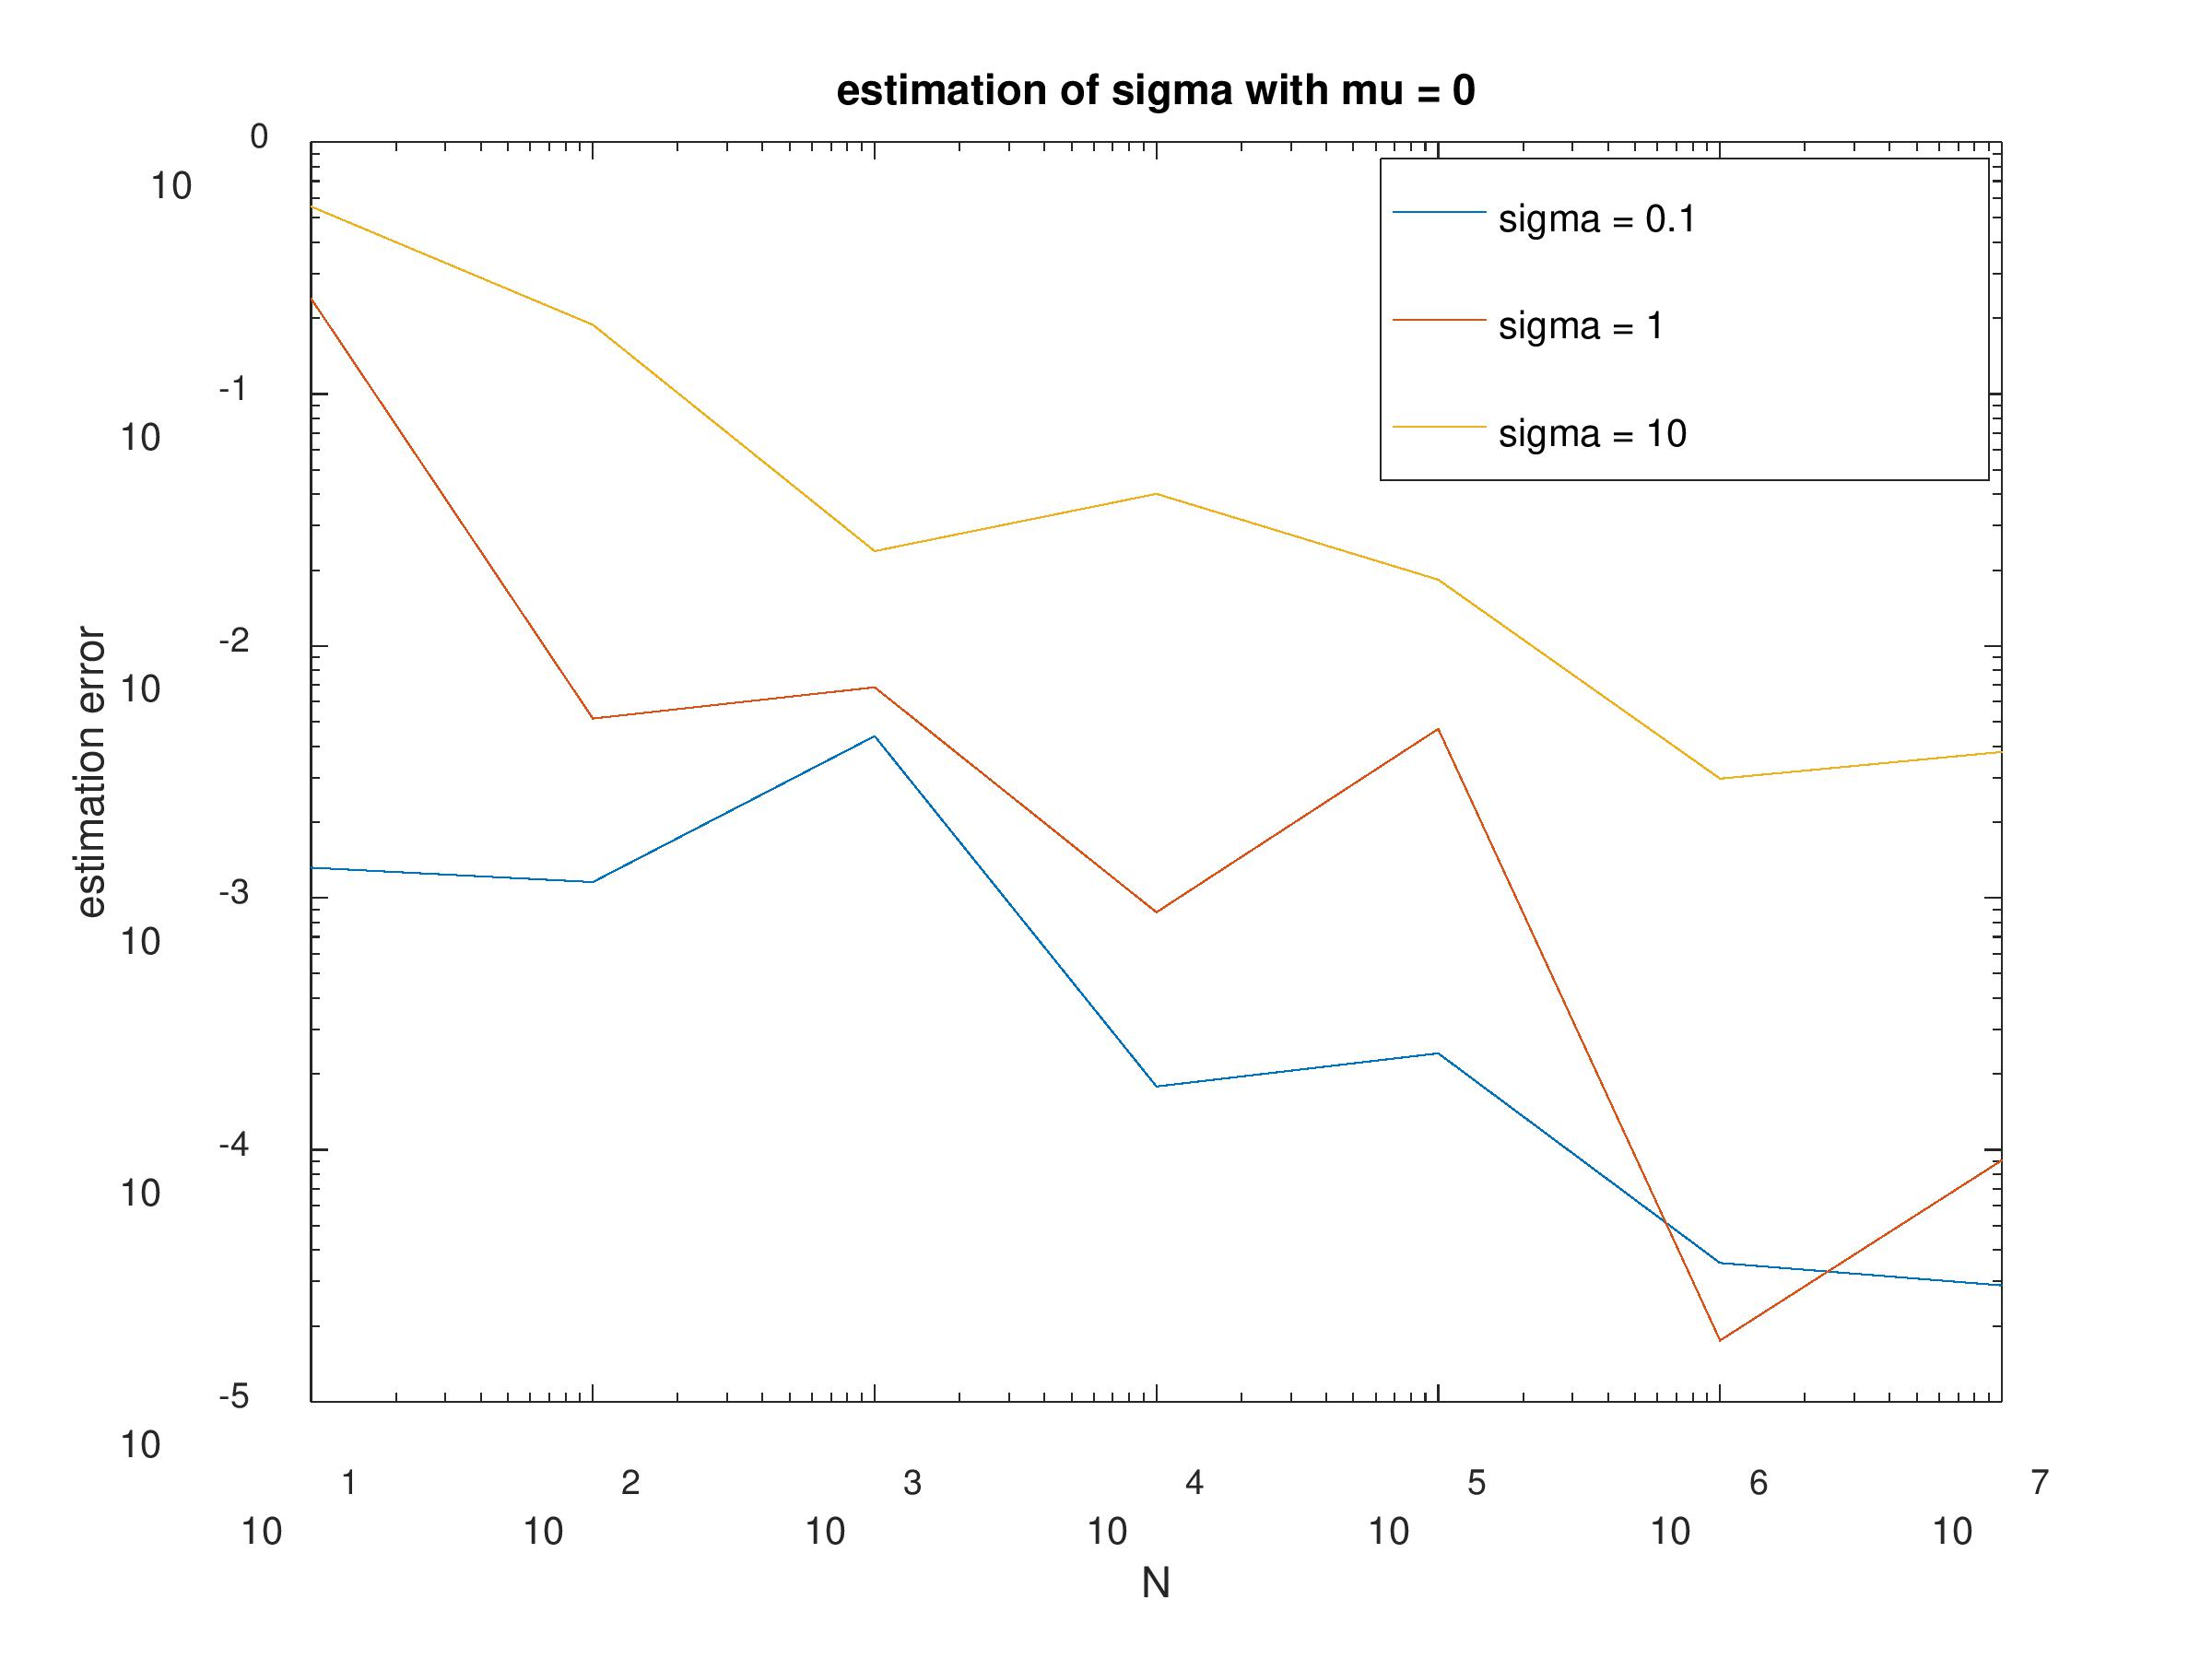
\includegraphics[scale=0.3]{sigma_err.jpeg}
\end{center}

\section*{Task 10}

\begin{center}
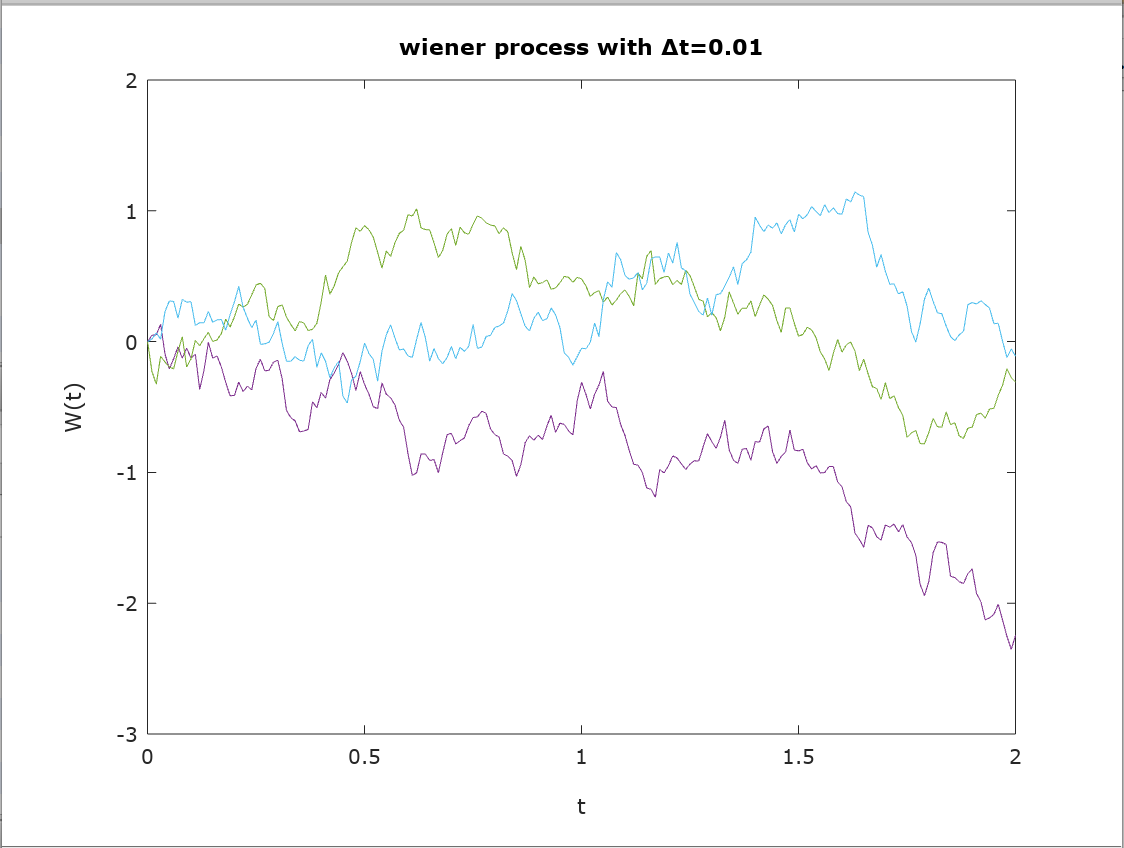
\includegraphics[scale=0.5]{wiener_001.jpeg}

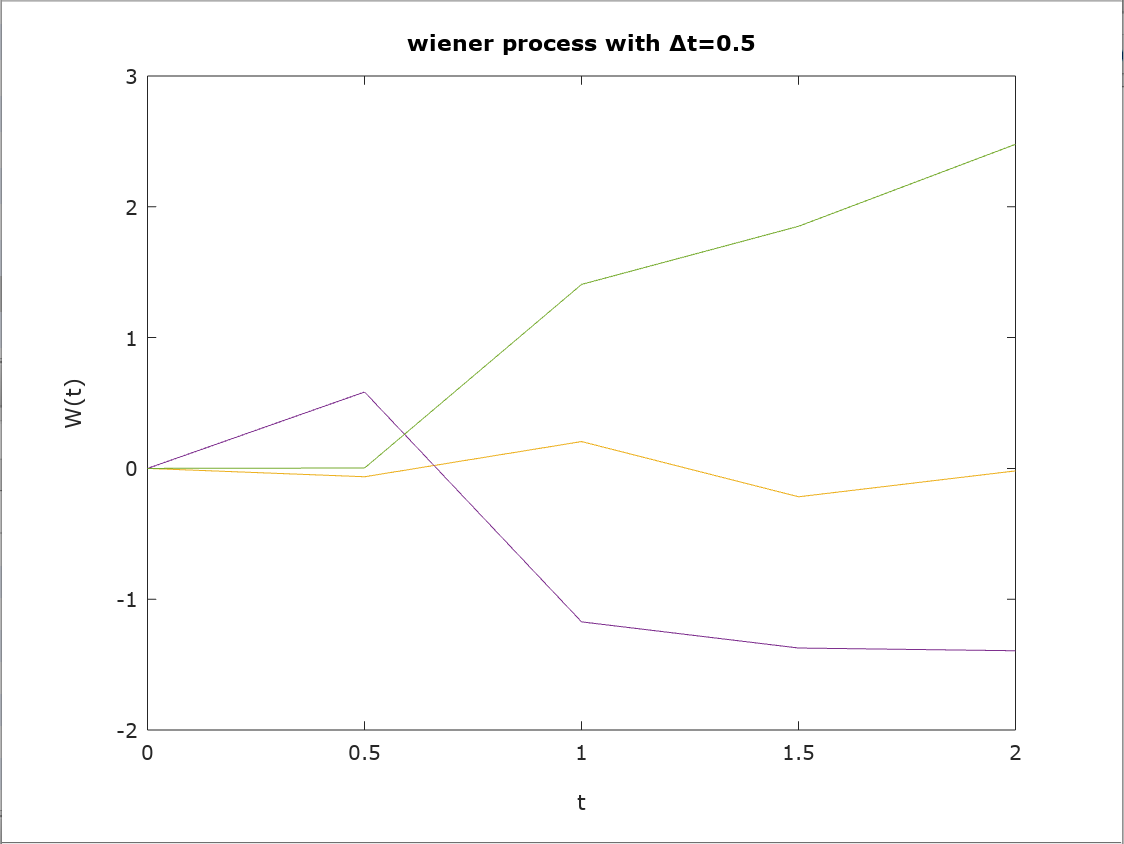
\includegraphics[scale=0.5]{wiener_05.jpeg}
\end{center}

\section*{Worksheet 2}

\section*{Task 1}

\begin{center}
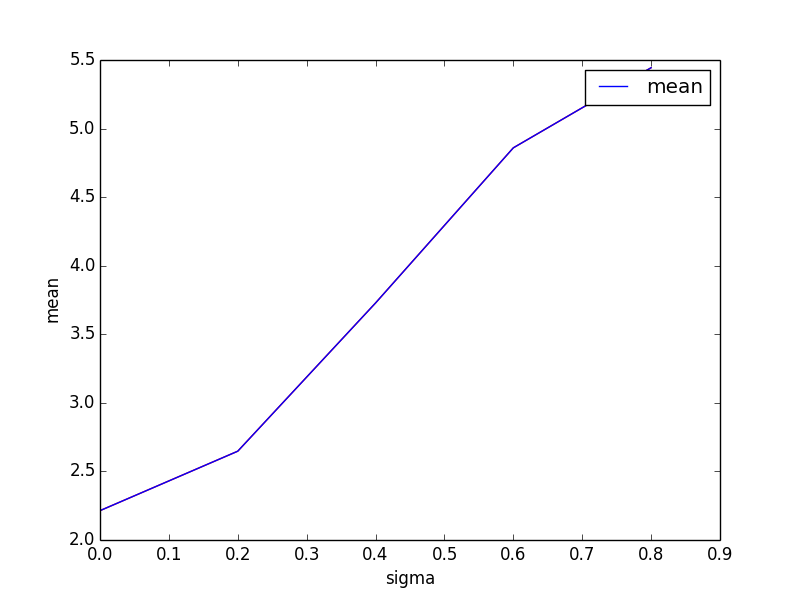
\includegraphics[scale=0.5]{task_1.png}		
\end{center}	

Obviously, increasing $\sigma$ leads to an increasing mean. This demonstrates, that with higher volatility, the fair price of the option increases as well (due to higher risk).

\section*{Task 2}

\begin{center}
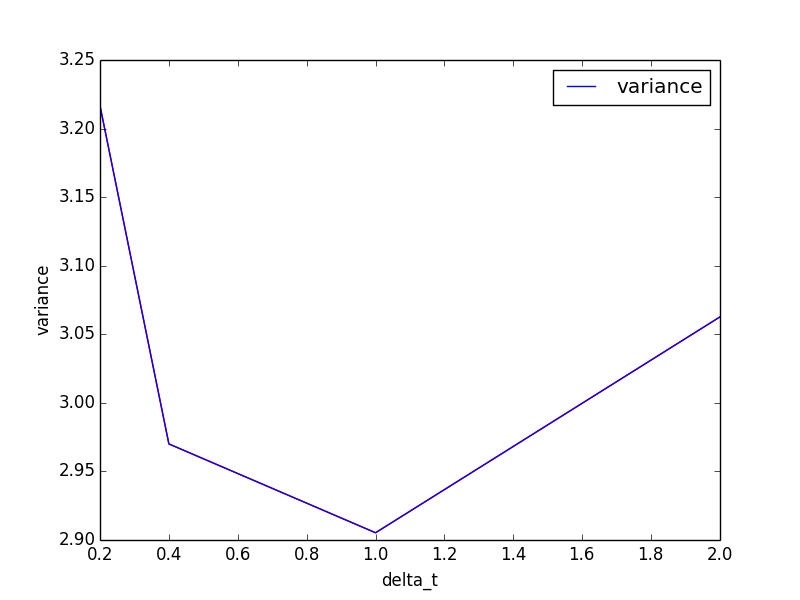
\includegraphics[scale=0.5]{task_2.png}		
\end{center}	

The variance is not affected by $\Delta t$, as this figure demonstrates. 

\section*{Task 3}
To prove that
\[
\mathbb{E}[V_{call}(S_T,0)]=S(0)\exp(\mu T)\Phi(\sigma\sqrt{T}-\chi)-K\Phi(-\chi)
\]
we use that by change-of-variable with $t:=-t$ we get
\begin{eqnarray}
&&\mathbb{E}[V_{call}(S_T,0)] \notag\\
&=&\frac{1}{\sqrt{2\pi}}\int_{\chi}^{\infty}\left(S(0)\exp\left((\mu-\frac{1}{2}\sigma^2)\cdot T+\sigma\sqrt{T}s\right)-K\right)\exp\left(-\frac{s^2}{2}\right)ds \notag\\
&=&\frac{1}{2\pi}\int_{\chi}^{\infty}\left(S(0)\exp\left((\mu-\frac{1}{2}\sigma^2)\cdot T+\sigma\sqrt{T}s\right)\right)\exp\left(-\frac{s^2}{2}\right)ds-K\frac{1}{2\pi}\int_{\chi}^{\infty}\exp\left(-\frac{t^2}{2}\right)dt \notag\\
&=&\Psi-K\frac{1}{2\pi}\int_{-\infty}^{-\chi}\exp\left(-\frac{t^2}{2}\right)dt \notag\\
&=&\Psi-K\Phi(-\chi) \notag
\end{eqnarray}
with
\[
\Psi:=\frac{1}{2\pi}\int_{\chi}^{\infty}\left(S(0)\exp\left((\mu-\frac{1}{2}\sigma^2)\cdot T+\sigma\sqrt{T}s\right)\right)\exp\left(-\frac{s^2}{2}\right)ds.
\]
Now we prove that
\[
\Psi=S(0)\exp(\mu T)\Phi(\sigma\sqrt{T}-\chi).
\]
Again, we use a change-of-variable $z:=t+\sigma\sqrt{T}$ and get
\begin{eqnarray}
&&\frac{1}{\sqrt{2\pi}}\exp\left(\frac{\sigma^2}{2}T\right)\int\limits_{-\infty}^{\sigma\sqrt{T}-\chi}\exp\left(-\frac{t^2}{2}\right)dt \notag\\
&=&\frac{1}{\sqrt{2\pi}}\exp\left(\frac{\sigma^2}{2}T\right)\int\limits_{\chi-\sigma\sqrt{T}}^{\infty}\exp\left(-\frac{t^2}{2}\right)dt \notag\\
&=&\frac{1}{\sqrt{2\pi}}\exp\left(\frac{\sigma^2}{2}T\right)\int\limits_{\chi}^{\infty}\exp\left(-\frac{(\sigma\sqrt{T}-z)^2}{2}\right)dz \notag\\
&=&\frac{1}{\sqrt{2\pi}}\int\limits_{\chi}^{\infty}\exp\left(-\frac{z^2}{2}+z\sigma\sqrt{T}\right)dz. \notag
\end{eqnarray}
We have
\begin{eqnarray}
\Psi&=&\frac{1}{\sqrt{2\pi}}S(0)\exp\left((\mu-\frac{\sigma^2}{2})\cdot T\right)\int_{\chi}^{\infty}\exp\left(-\frac{s^2}{2}+\sigma\sqrt{T}s\right)ds \notag\\
&=&S(0)\exp(\mu T)\exp\left(-\frac{\sigma^2}{2}T\right)\frac{1}{\sqrt{2\pi}}\int_{\chi}^{\infty}\exp\left(-\frac{s^2}{2}+\sigma\sqrt{T}s\right)ds \notag\\
&=&S(0)\exp(\mu T)\frac{1}{\sqrt{2\pi}}\exp\left(-\frac{\sigma^2}{2}T\right)\exp\left(\frac{\sigma^2}{2}T\right)\int\limits_{-\infty}^{\sigma\sqrt{T}-\chi}\exp\left(-\frac{s^2}{2}\right)ds \notag\\
&=&S(0)\exp(\mu T)\Phi(\sigma\sqrt{T}-\chi). \notag
\end{eqnarray}

\section*{Task 4}

\begin{center}
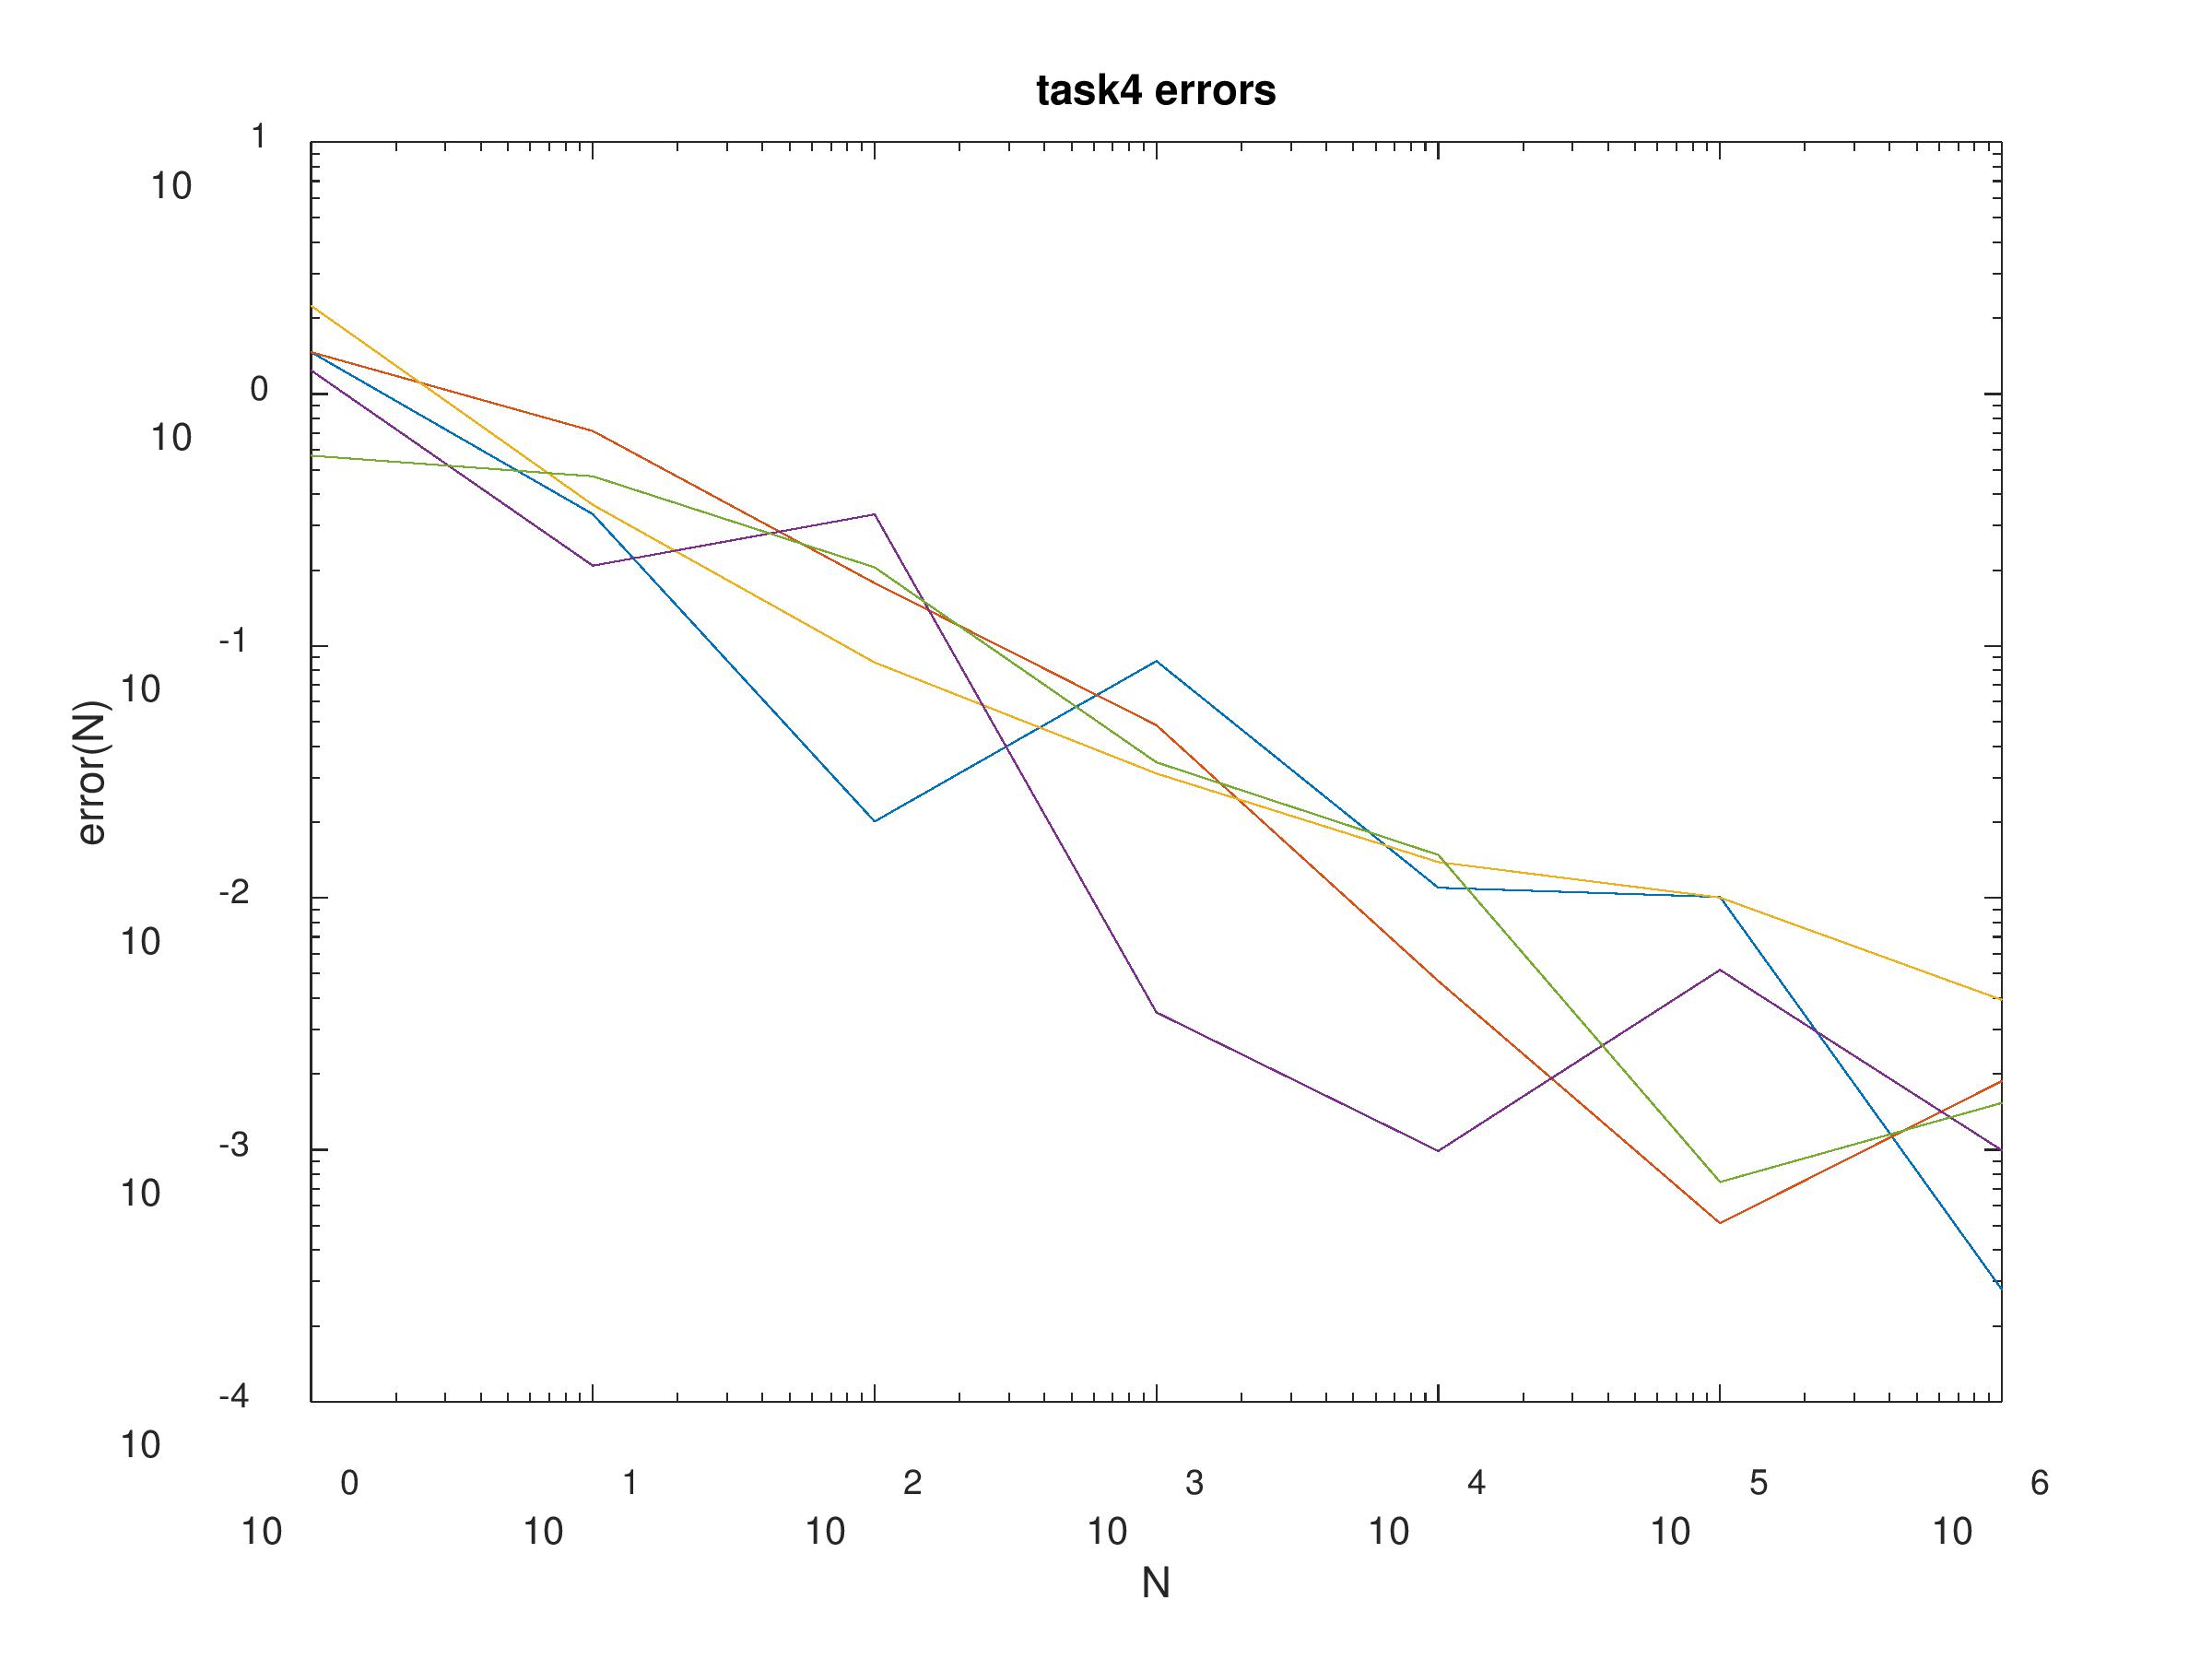
\includegraphics[scale=0.3]{task4.jpg}		
\end{center}	

$5$ independent simulations of $\mathbb{E}[V_{call}(S_T,0)]$. As expected, the rate of convergence is $O(N^{-1/2})$.

\section*{Task 5}
We have $\Phi^{-1}(0)=-\infty$ and $\Phi^{-1}(1)=\infty$ where $\Phi^{-1}:(0,1)\to(-\infty,\infty)$ is the inverse cumulative distribution function. As an integral of a positive continious function, $\Phi$ is a bijection, continious and differentiable. That means $\Phi$ is a diffeomorphism. $\Phi^{-1}$ is also differentiable, so we can use the transformation theorem with the change-of-variable $t=\Phi(s)$. We have $|\det(D\Phi(s))|=\frac{1}{\sqrt{2\pi}}\exp(-\frac{s^2}{2})$ and
\begin{eqnarray}
&&\int_0^1 f(\Phi^{-1}(t))dt \notag\\
&=&\int_{\Phi^{-1}(0)}^{\Phi^{-1}(1)}f(\Phi^{-1}(\Phi(s)))\cdot|\det(D\Phi(s))|ds \notag\\
&=&\int_{-\infty}^{\infty}f(s)\frac{1}{\sqrt{2\pi}}\exp\left(-\frac{s^2}{2}\right)ds \notag\\
&=&\frac{1}{\sqrt{2\pi}}\int_{-\infty}^{\infty}f(s)\exp\left(-\frac{s^2}{2}\right)ds \notag
\end{eqnarray}
what proves formula (7).

\section*{Task 6}

In case of the trapezoidal-rule, the set of nodes of level $l$ is a subset of the nodes of level $l+1$. Furthermore, the $2^l$ additional values lay exactly half way in between the nodes of level $l$. (Except for the first and the last node, which lie half way in between 0 and the first node of level $l$ and in between the last node of level $l$ and the end of the interval.) 

\section*{Task 7}

In case of the Gauß-Legendre Quadrature, the nodes of level $l$ are not a subset of the nodes of level $l+1$. At the edges of the interval, the nodes are denser. According to Satz 1.18 from Einführung in die Grundlagen der Numerik, node $x_i^{(N_l)}$ from level $l$ lays between the nodes $x_i^{(N_{l+1})}, x_{i+1}^{(N_{l+1})}$ from level $l+1$.

The nodes are the roots of a three-term-recurrence relation of the form $p_{n+1}(t)=(t-\alpha_n)p_n(t)-\beta_n^2p_{n-1}(t)$, $n \geq 0$. 
The roots are the eigenvalues of a tridiagonal $(N_l \times N_l)$-dimensional matrix of the form

\begin{align*}
\begin{bmatrix}
\alpha_0 &  \beta_1  & 0 & ... & ... & ... \\
\beta_1 & \alpha_1 & \beta_2 & ... & ... & ... \\
 0  & \beta_2 & a_2 & \beta_3 & ... & ... \\
0   & ... & ... & ... & ... & 0 \\
... & ... &  0  & \beta_{N_l-2} & \alpha_{N_l-2} & \beta_{N_l-1}  \\
... & ... & ... & 0  & \beta_{N_l-1} & \alpha_{N_l-1} \\
\end{bmatrix}
\end{align*}



The weights are the first entry of the eigenvectors to the eigenvalues calculated for the nodes. Alternitavely, they can be recieved by taking $\Lambda_{n+1}(x_i)$ of the Christoffel-function, with $x_i, i=1,...,n$ nodes. 



\section*{Task 8}

The Clenshaw-Curtis Quadrature rule uses nested nodes, the nodes of each level are a subset of the nodes of higher levels. Similarly to Gauß-Legendre quadrature, the number of nodes is higher at the edges of the interval. 

\section*{Task 9}

\begin{center}
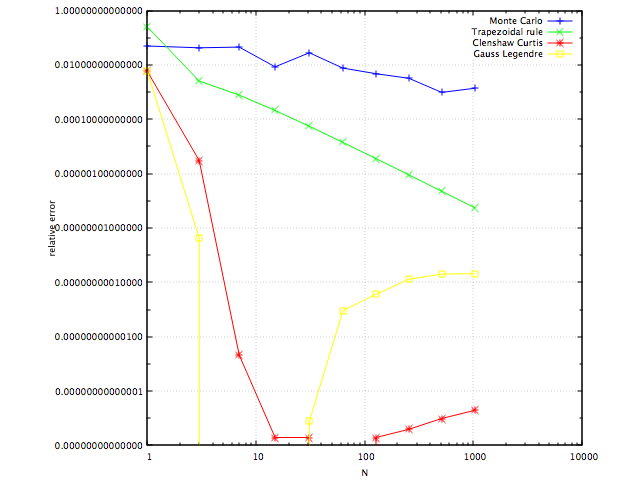
\includegraphics[scale=0.5]{task_9.png}		
\end{center}	

\section*{Task 10}

For $K=0$:
\begin{center}
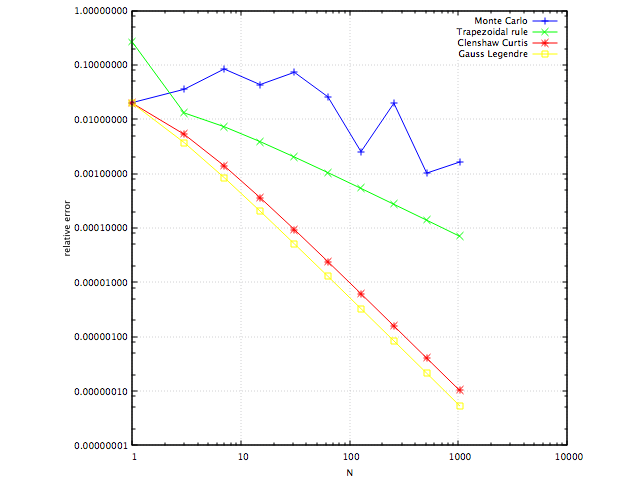
\includegraphics[scale=0.5]{relative_errors_K0.png}		
\end{center}	

\newpage

For $K=10$:
\begin{center}
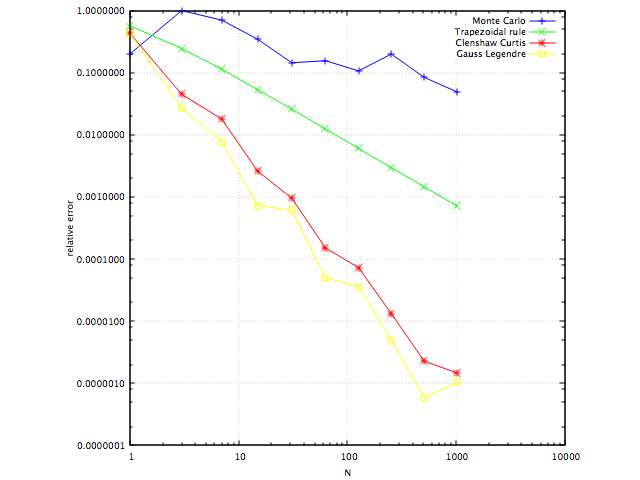
\includegraphics[scale=0.5]{relative_errors_K10.png}		
\end{center}	


%Sheet 3

\section*{Worksheet 3}

\section*{Task 3}

\begin{center}
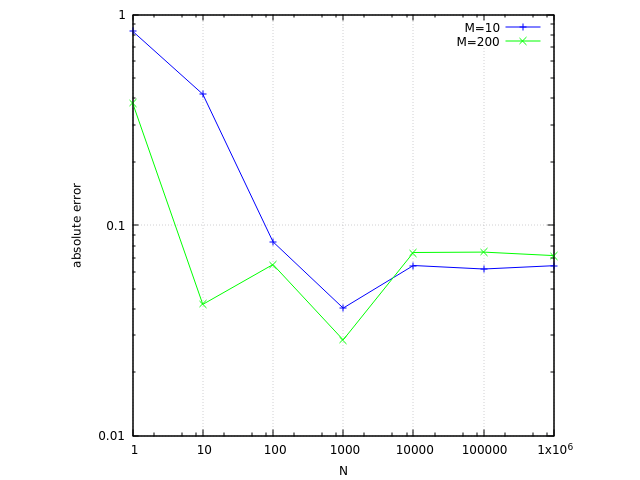
\includegraphics[scale=0.5]{error_task_3.png}
\end{center}
The number of timesteps is not really effecting the convergence.

\section*{Task 4}

\begin{center}
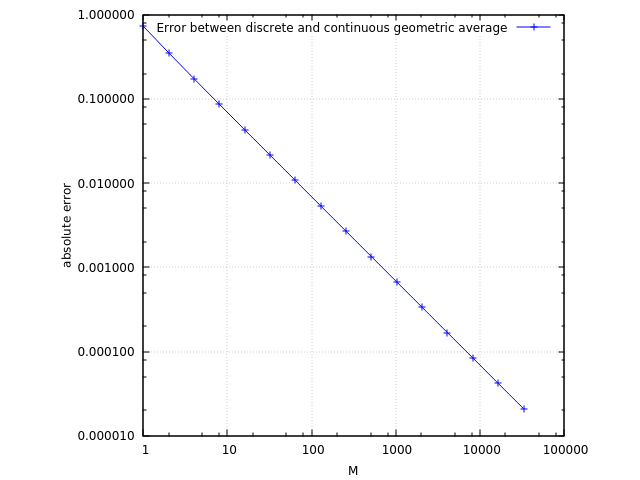
\includegraphics[scale=0.5]{error_continuous_discrete.png}		
\end{center}
The discrete geometric average converges linearly to the continuous geometric average.

\section*{Task 5}

\begin{center}
%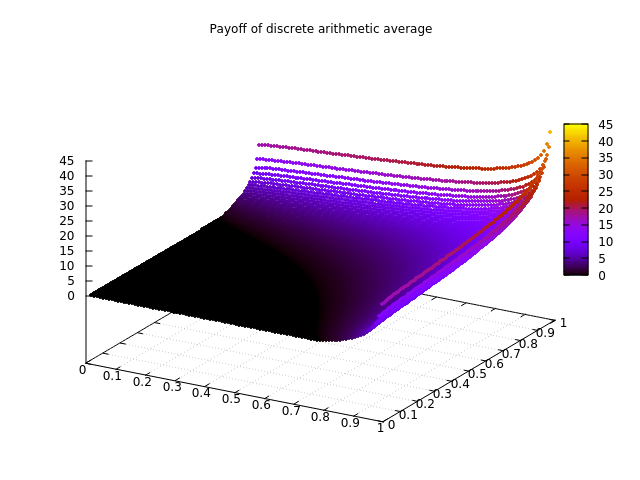
\includegraphics[scale=0.5]{payoff_discrete_arithmetic_average.png}
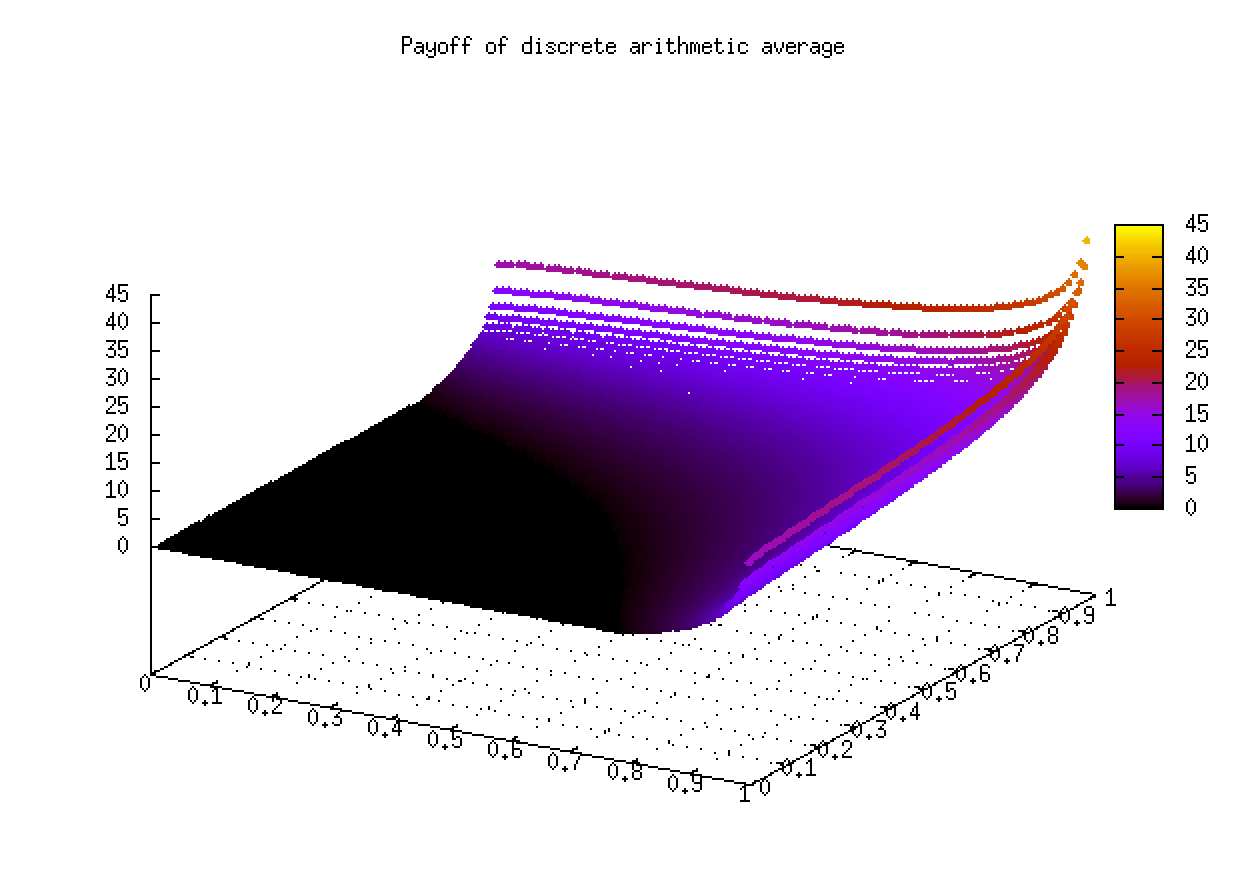
\includegraphics[scale=0.5]{s3t5.png}
\end{center}
The discrete geometric payoff function is evaluated on 10.000 points in $[0,1]^2$.

\newpage
\section*{Task 7}

Uniform random numbers in $(0,1)^2$:
\begin{center}
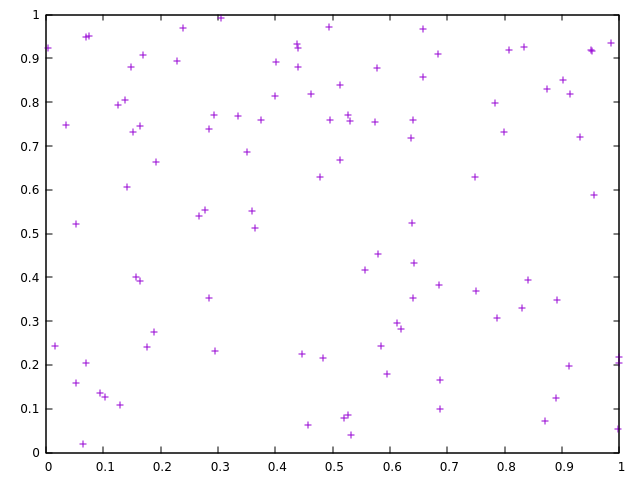
\includegraphics[scale=0.5]{uniform_random_numbers.png}		
\end{center}

Halton sequence:
\begin{center}
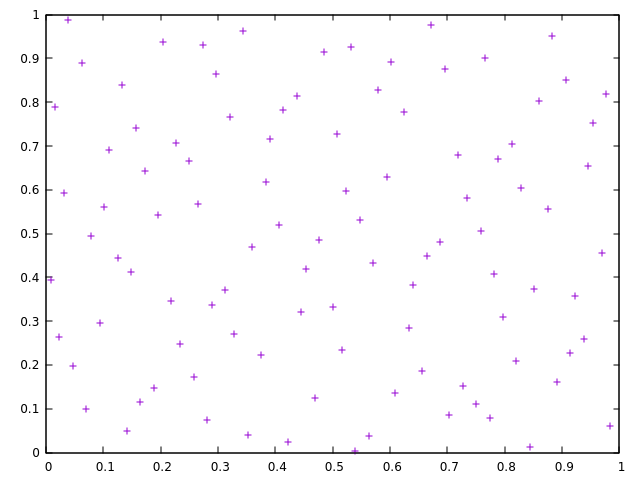
\includegraphics[scale=0.5]{halton_sequence.png}		
\end{center}

One can see that there are some regions in $(0,1)^2$ where no uniform random numbers are set. This is not the case in the point set calculated by the Halton sequence. The Halton sequence gives a very uniform spread set without any holes.

\newpage
\section*{Task 9}

Quadrature nodes of the two-dimensional product rule for trapezoidal rule:
\begin{center}
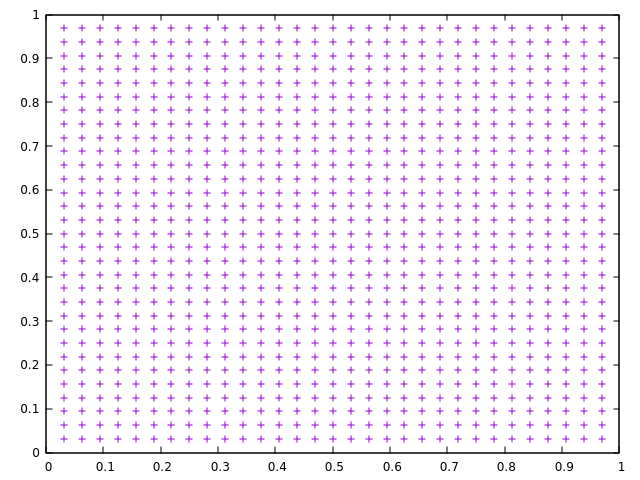
\includegraphics[scale=0.5]{quadrature_nodes_trapezoidal_rule.png}		
\end{center}

Quadrature nodes of the two-dimensional product rule for Gauss-Legendre:
\begin{center}
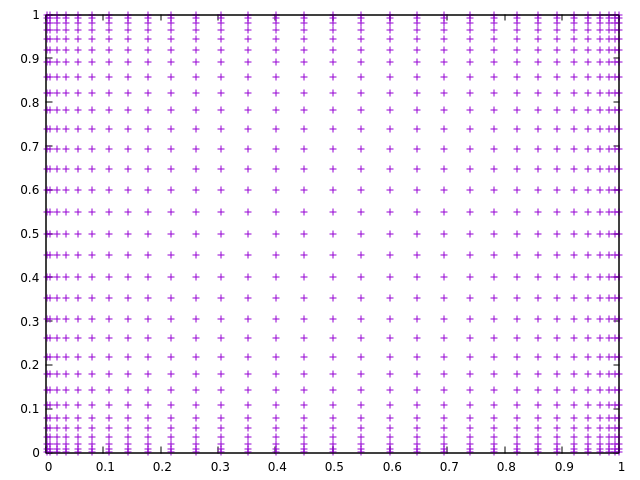
\includegraphics[scale=0.5]{quadrature_nodes_gauss_legendre.png}		
\end{center}
\newpage
Quadrature nodes of the two-dimensional product rule for Clenshaw Curtis:
\begin{center}
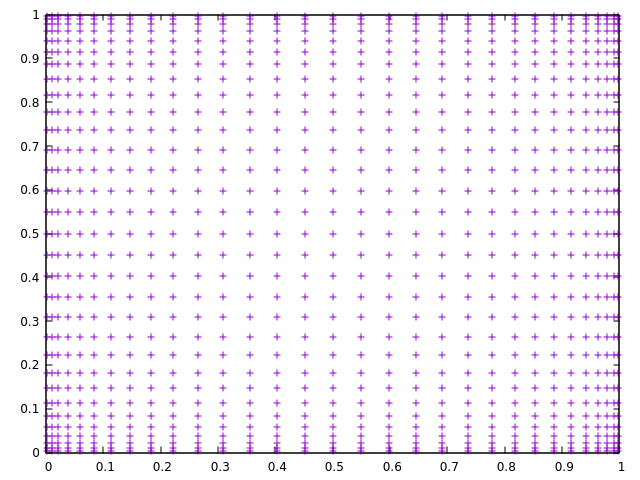
\includegraphics[scale=0.5]{quadrature_nodes_clenshaw_curtis.png}		
\end{center}

Both Gauß-Quadrature and Clenshaw-Curtis-Quadrature have an increased amount of nodes at the edges of the integration region. The trapeziodal rule distributes the nodes equidistantly over the integration region.

\section*{Task 11}

Two-dimensional Sparse Grid using Trapeziodal Rule for $l=5$:
\begin{center}
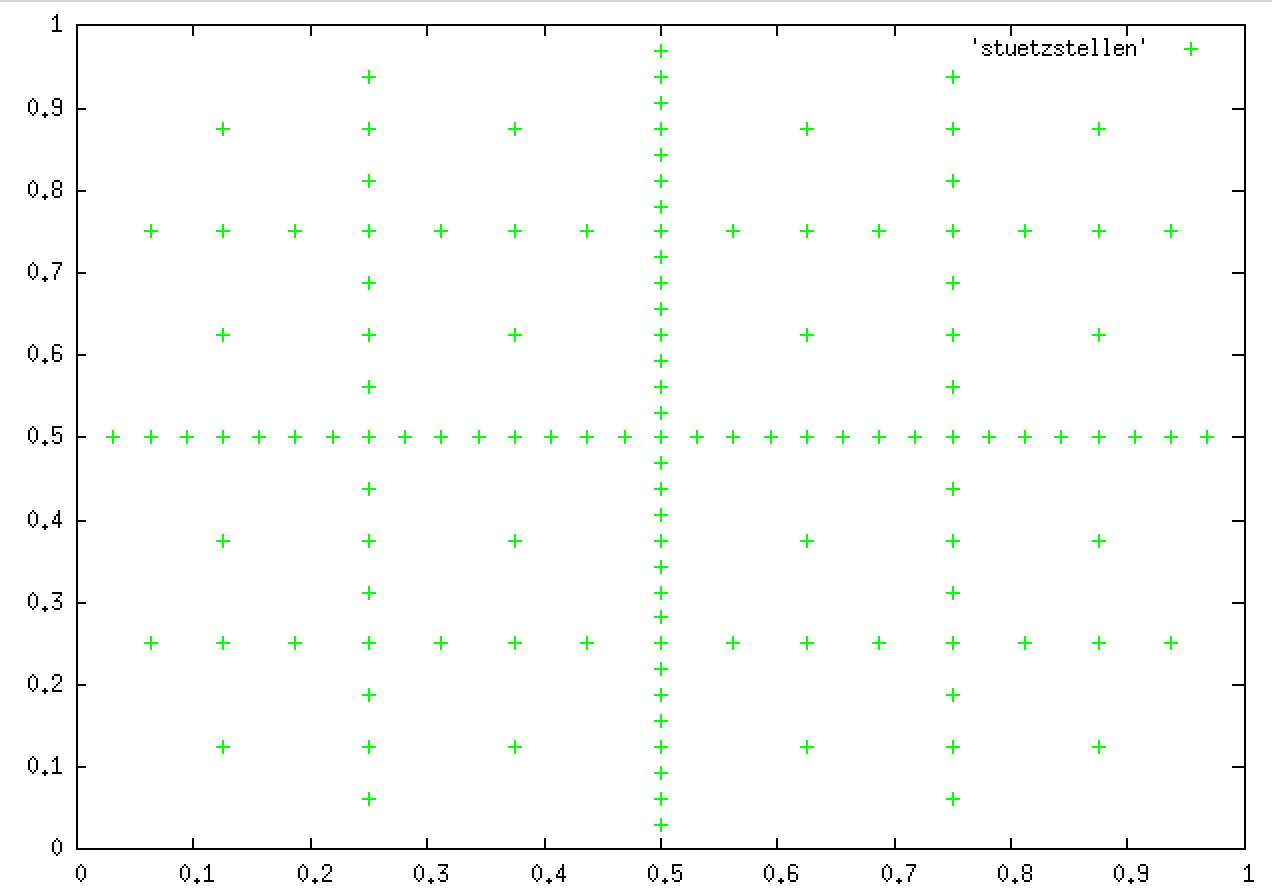
\includegraphics[scale=0.5]{sparse_grid_l5.png}	
\end{center}
\newpage
Two-dimensional Sparse Grid using Trapezoidal Rule for $l=7$:
\begin{center}
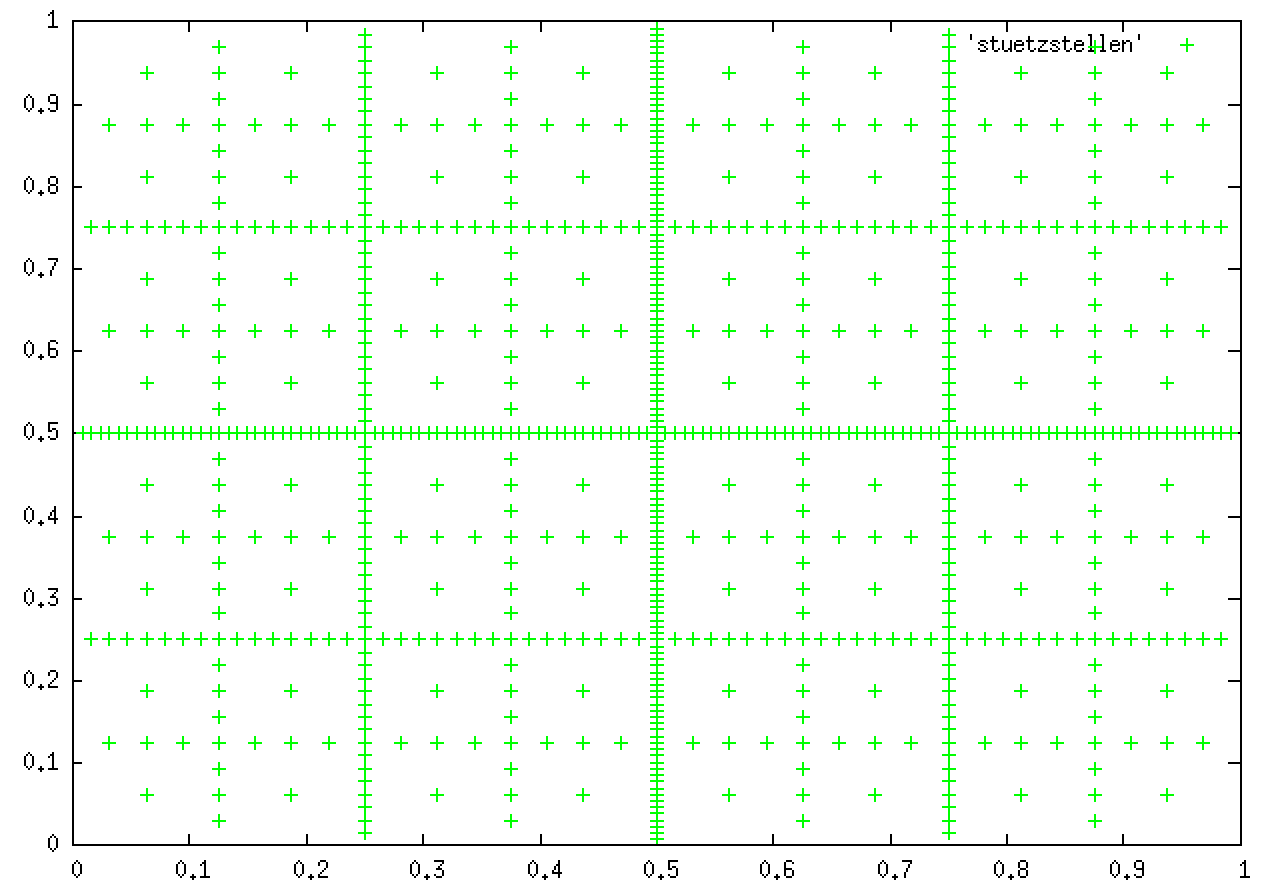
\includegraphics[scale=0.5]{sparse_grid_l7.png}	
\end{center}

Two-dimensional Sparse Grid using Clenshaw-Curtis Quadrature Rule for $l=5$:
\begin{center}
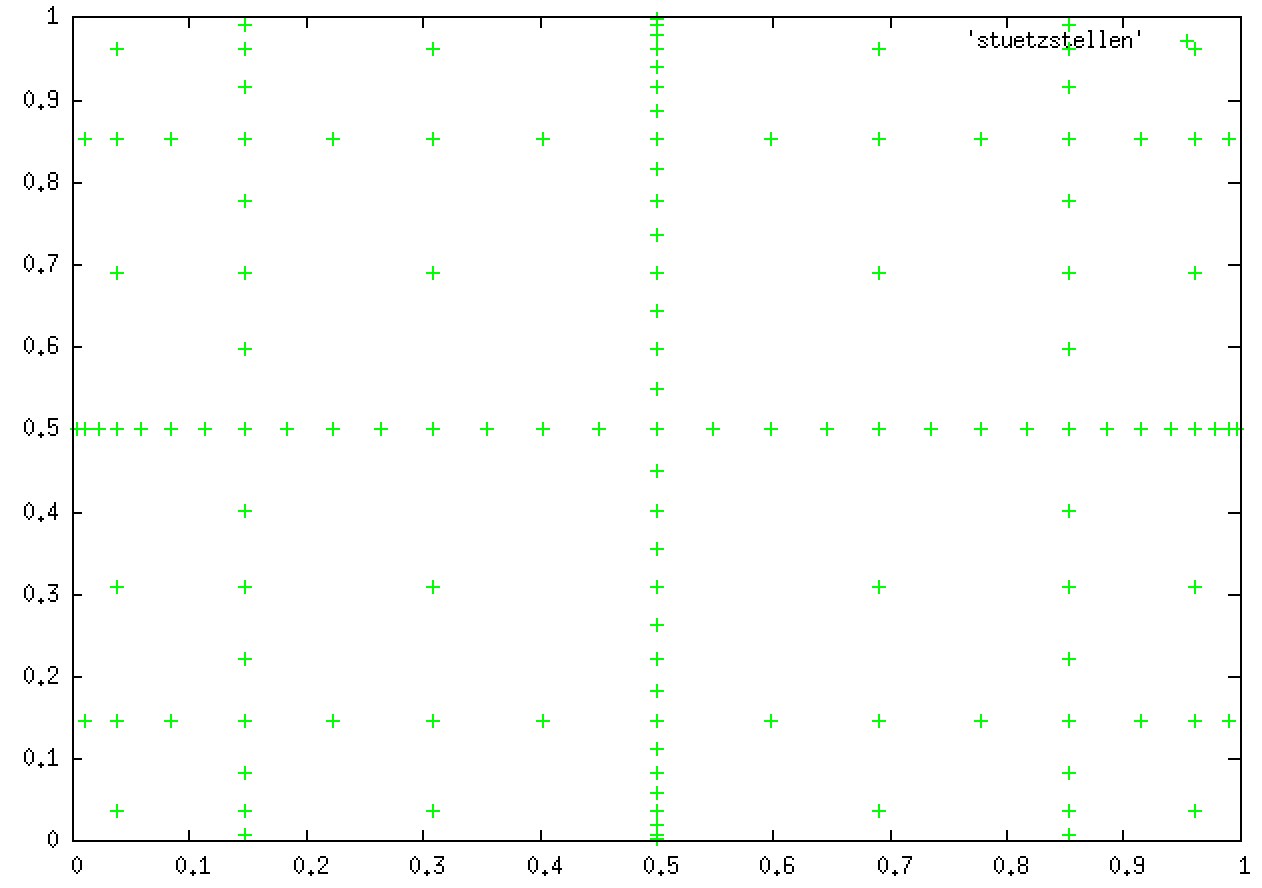
\includegraphics[scale=0.5]{clenshaw_curtis_l5.png}	
\end{center}
\newpage
Two-dimensional Sparse Grid using Clenshaw-Curtis Quadrature Rule for $l=7$:
\begin{center}
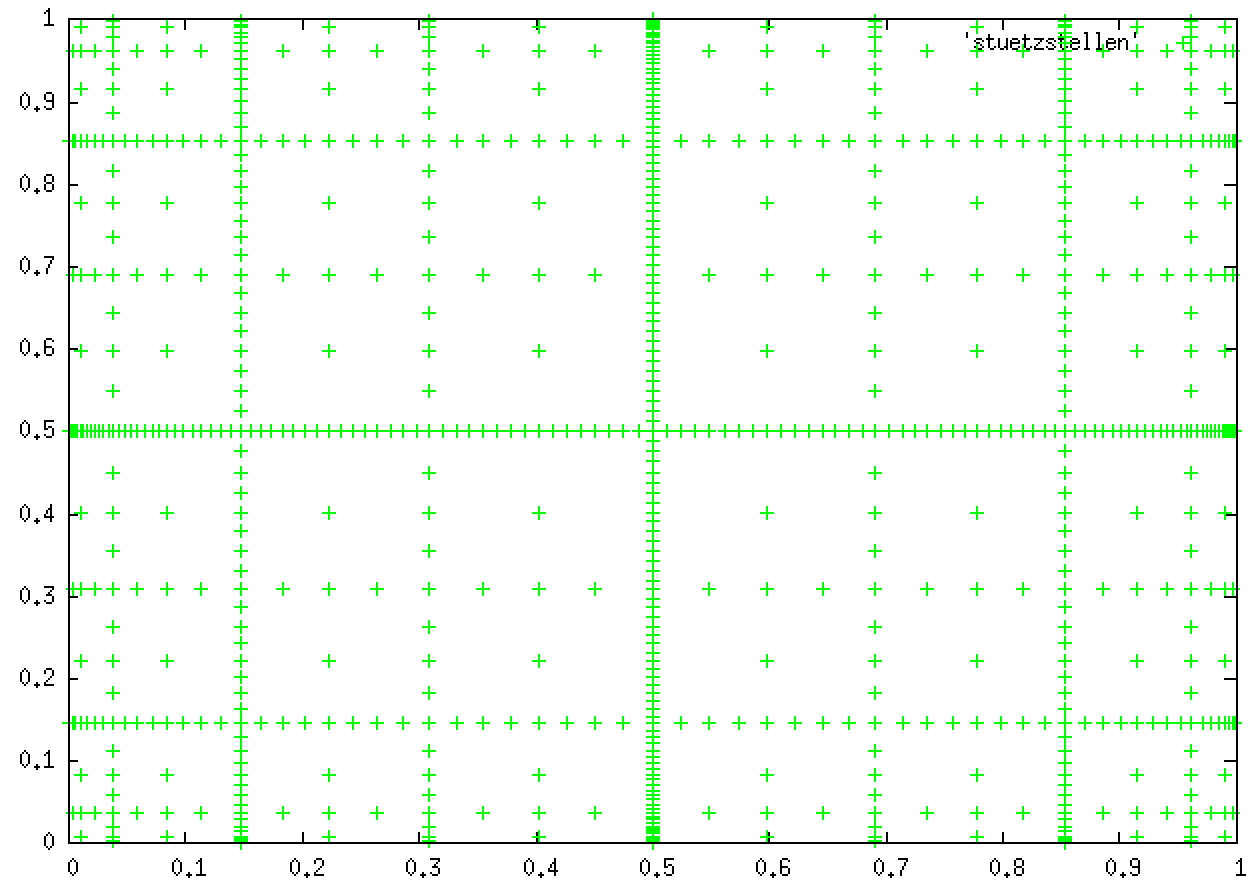
\includegraphics[scale=0.5]{clenshaw_curtis_l7.png}	
\end{center}
For Clenshaw-Curtis Quadrature, with increasing level, more nodes are situated at the edges of the integration region. For Trapezoidal Rule, this is not the case.

\newpage
\section*{Task 12}

Number of points in Sparse Grid and Full Grid in Level $l=4$:
\begin{center}
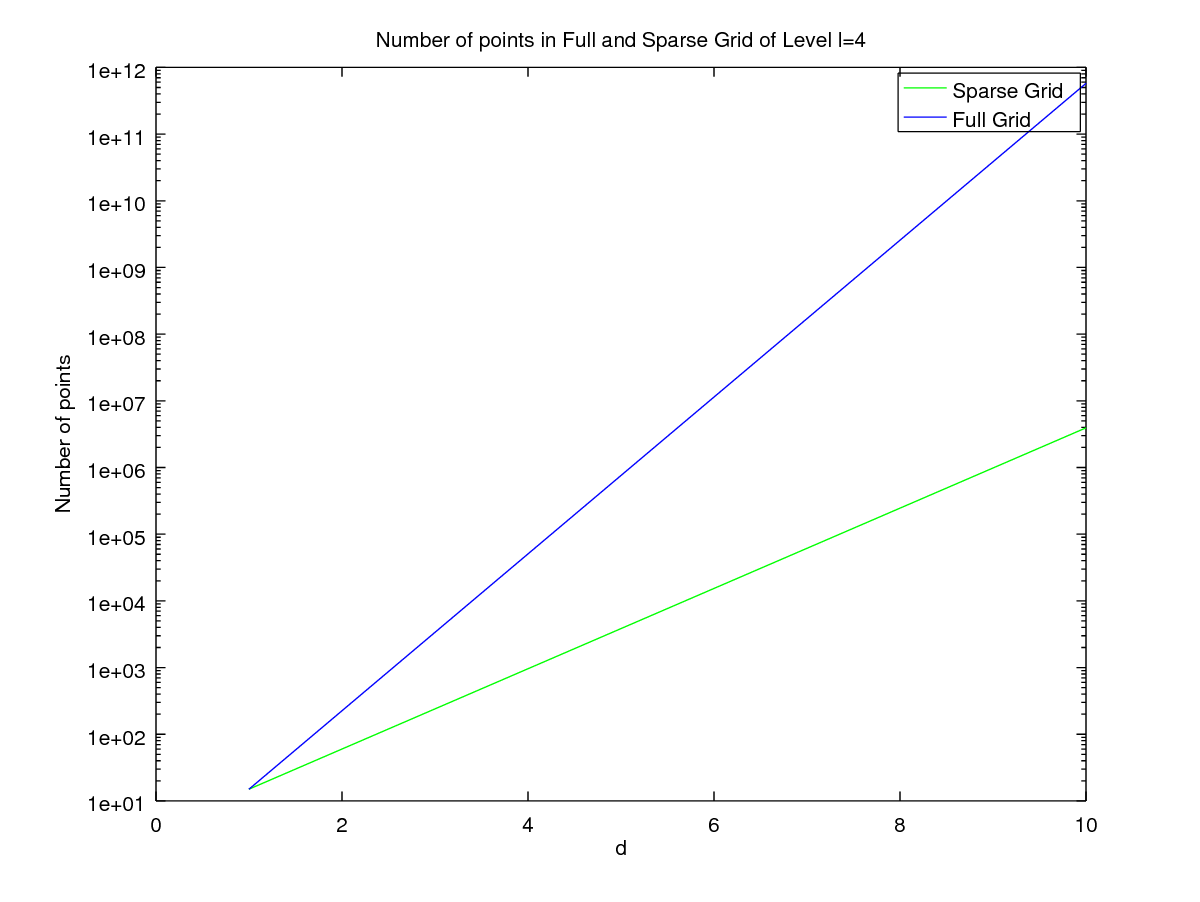
\includegraphics[scale=0.5]{number_of_points_SG_FG.png}
\end{center}
One can see that the number of points increases much faster in the Full Grid than in the Sparse Grid.

\section*{Task 13}

Convergence plots for the testfunction $f_\gamma$ in different dimensions:
\begin{center}
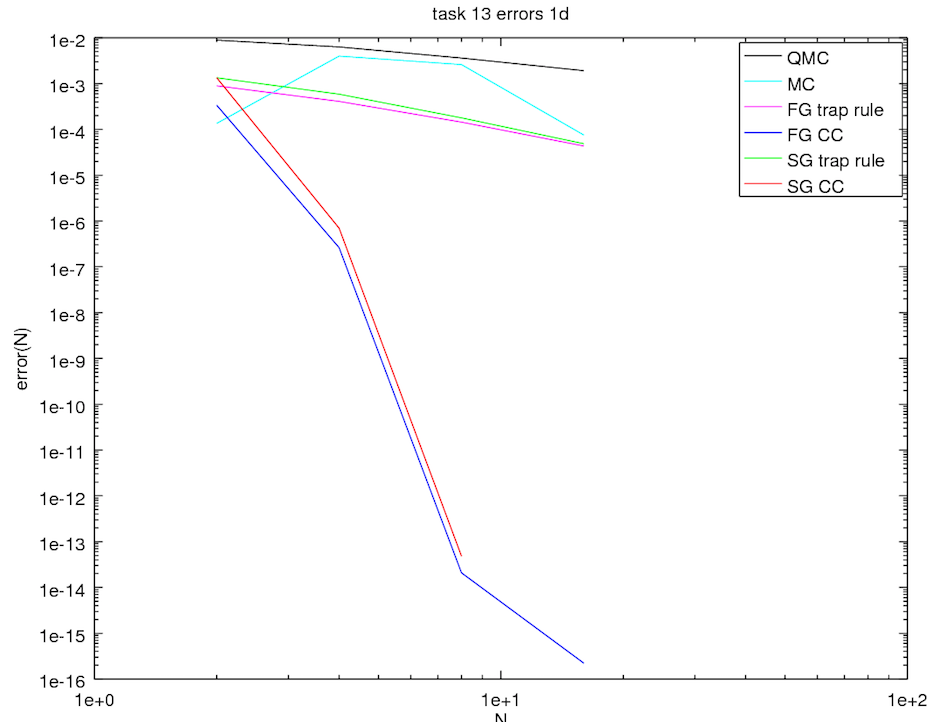
\includegraphics[scale=0.5]{task_13_d1.png}
\end{center}
\begin{center}
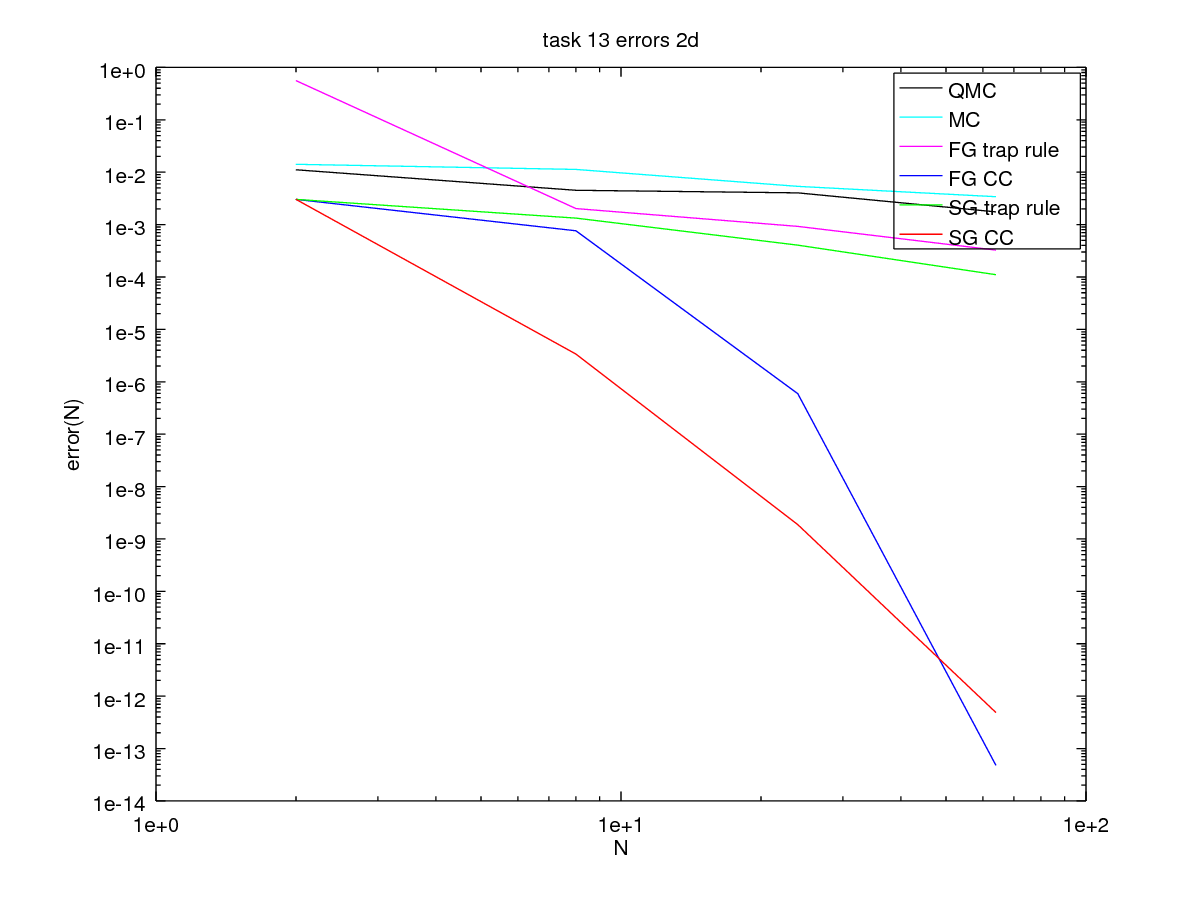
\includegraphics[scale=0.5]{task_13_d2.png}
\end{center}
\begin{center}
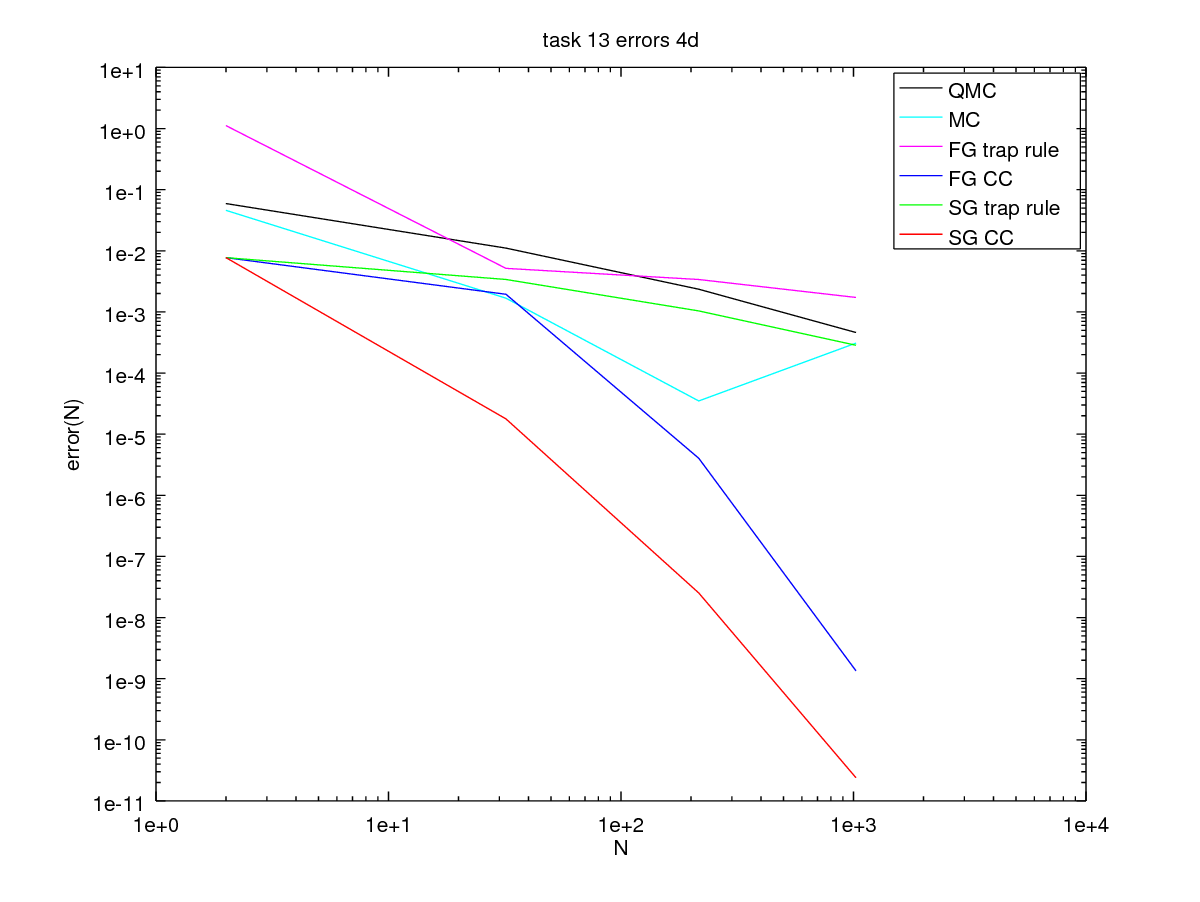
\includegraphics[scale=0.5]{task_13_d4.png}
\end{center}
\begin{center}
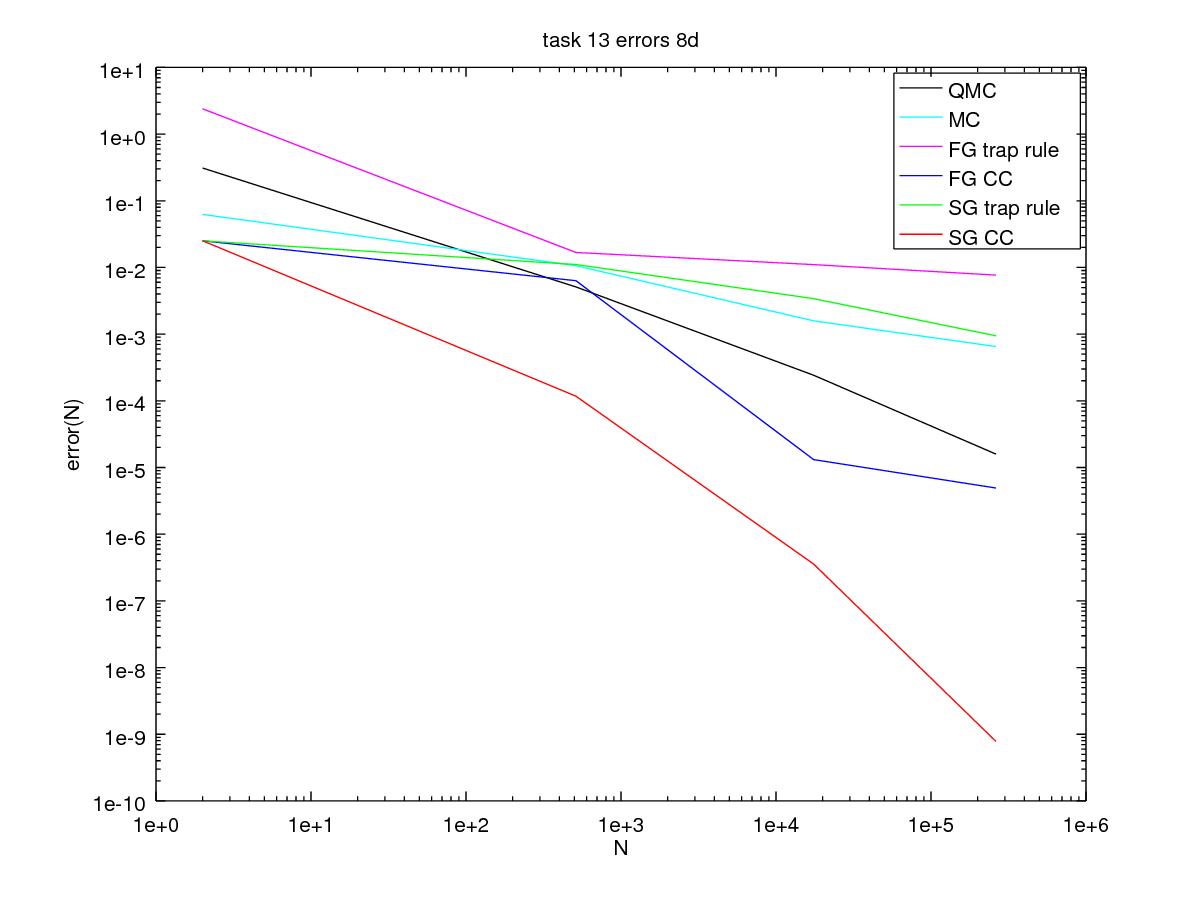
\includegraphics[scale=0.5]{task_13_d8.png}
\end{center}
Obviously, the Sparse Grid Method has the best convergence and the Full
Grid method has the second best convergence, while MC and QMC can't match
these convergence rates. Since the quadrature nodes are better distributed on
the integration region, QMC has better convergence than MC.

\section*{Task 15}
\begin{center}
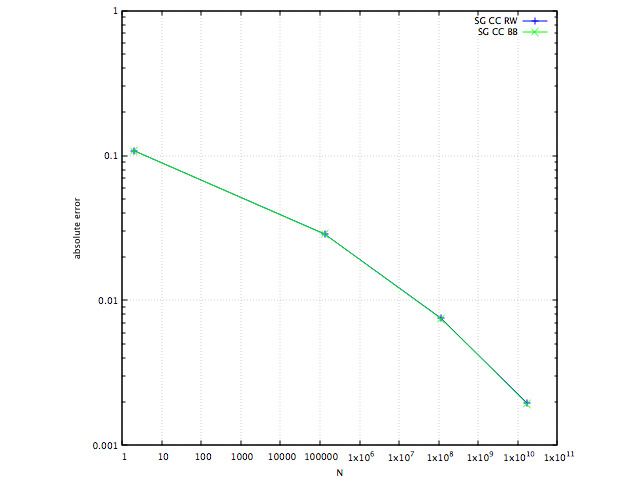
\includegraphics[scale=0.5]{task15.png}
\end{center}

Here, since the payoff function isn't sufficiently smooth for Clenshaw-Curtis to work properly, the Brownian Bridge Method shows no advantage in convergence over Random Walk. 

\section*{Task 16}
\begin{center}
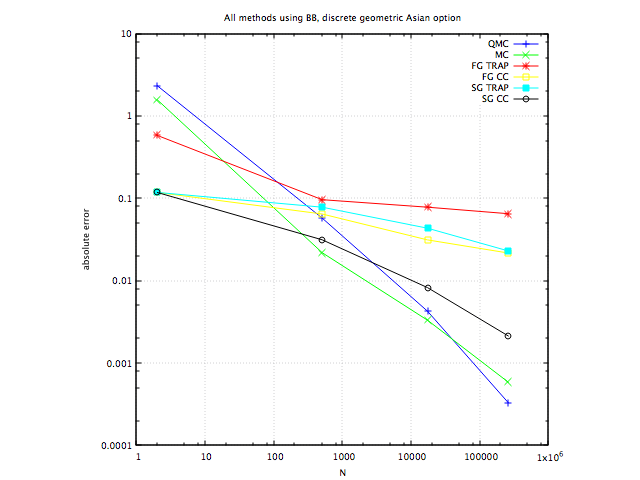
\includegraphics[scale=0.5]{task16bb.png}
\end{center}
\begin{center}
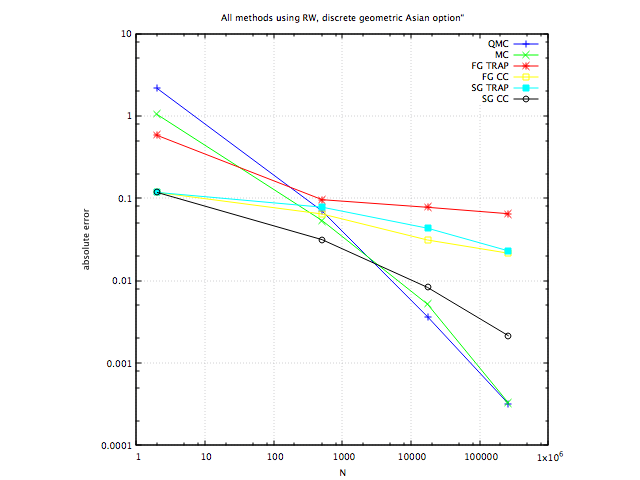
\includegraphics[scale=0.5]{task16rw.png}
\end{center}
In this case, due to lack of smoothness, Monte Carlo and Quasi Monte Carlo perform better than more sophisticated quadrature rules. 
\section*{Task 17}
\begin{center}
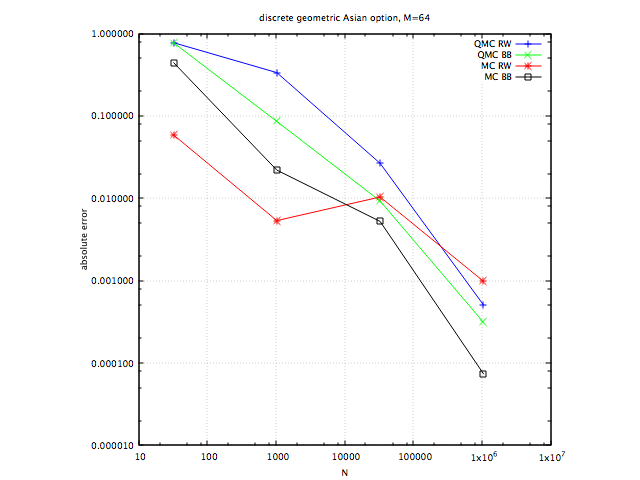
\includegraphics[scale=0.42]{task17.png}
\end{center}
This illustrates the superiority of Brownian Bridge Interpolation over
Random Walk for Monte Carlo and Quasi Monte Carlo integration. 

\section*{Task 18}

The difference between MC and QMC is, that MC uses actual pseudo random numbers, while QMC uses deterministic sequences. For this reason, QMC Quadrature Nodes are more evenly distributed over the integration region, which enhances the convergence rate of QMC (which is $\mathcal{O}(N)$) compared to the convergence of $\mathcal{O}(N^{1/2})$ of Monte Carlo Method. However, there is a higher computational effort in creating quasi-random-number sequences, which increases the cost of QMC especially in high dimensions compared to Monte Carlo. \\

Both, QMC and MC, can integrate a wide range of functions, regardless of how smooth these functions are. \\

Sparse Grids and Full Grids make use of nodes and weights which result from quadrature methods like Clenshaw-Curtis or Trapezoidal rule. These methods can only be applied to somewhat smoother functions, but they have much better convergence rates. 
Full Grids are heavily affected by the dimension, with the number of nodes increasing exponentially with increasing dimension. For sparse grids, dependence on dimension is considerably lower. \\

Therefore, if it is known that the integrand will be relatively smooth, using Sparse Grid methods is the best way to compute integrals in high dimensions. However, if the integrand is unknown or if the integrand is a function that is not differentiable in many points, MC and QMC integration are the preferred methods, espacially in high dimensions.

%Sheet 4
\section*{Worksheet 4}

\section*{Task 1}

\begin{center}
	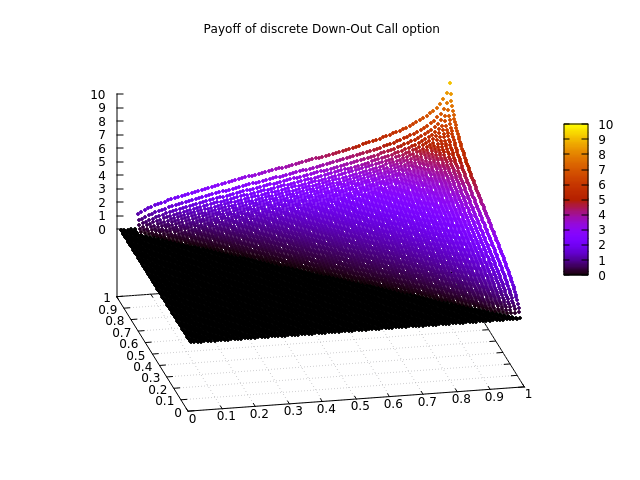
\includegraphics[scale=0.7]{images/payoff_down_out_call.png}
\end{center}

\section*{Task 2}


\begin{center}
	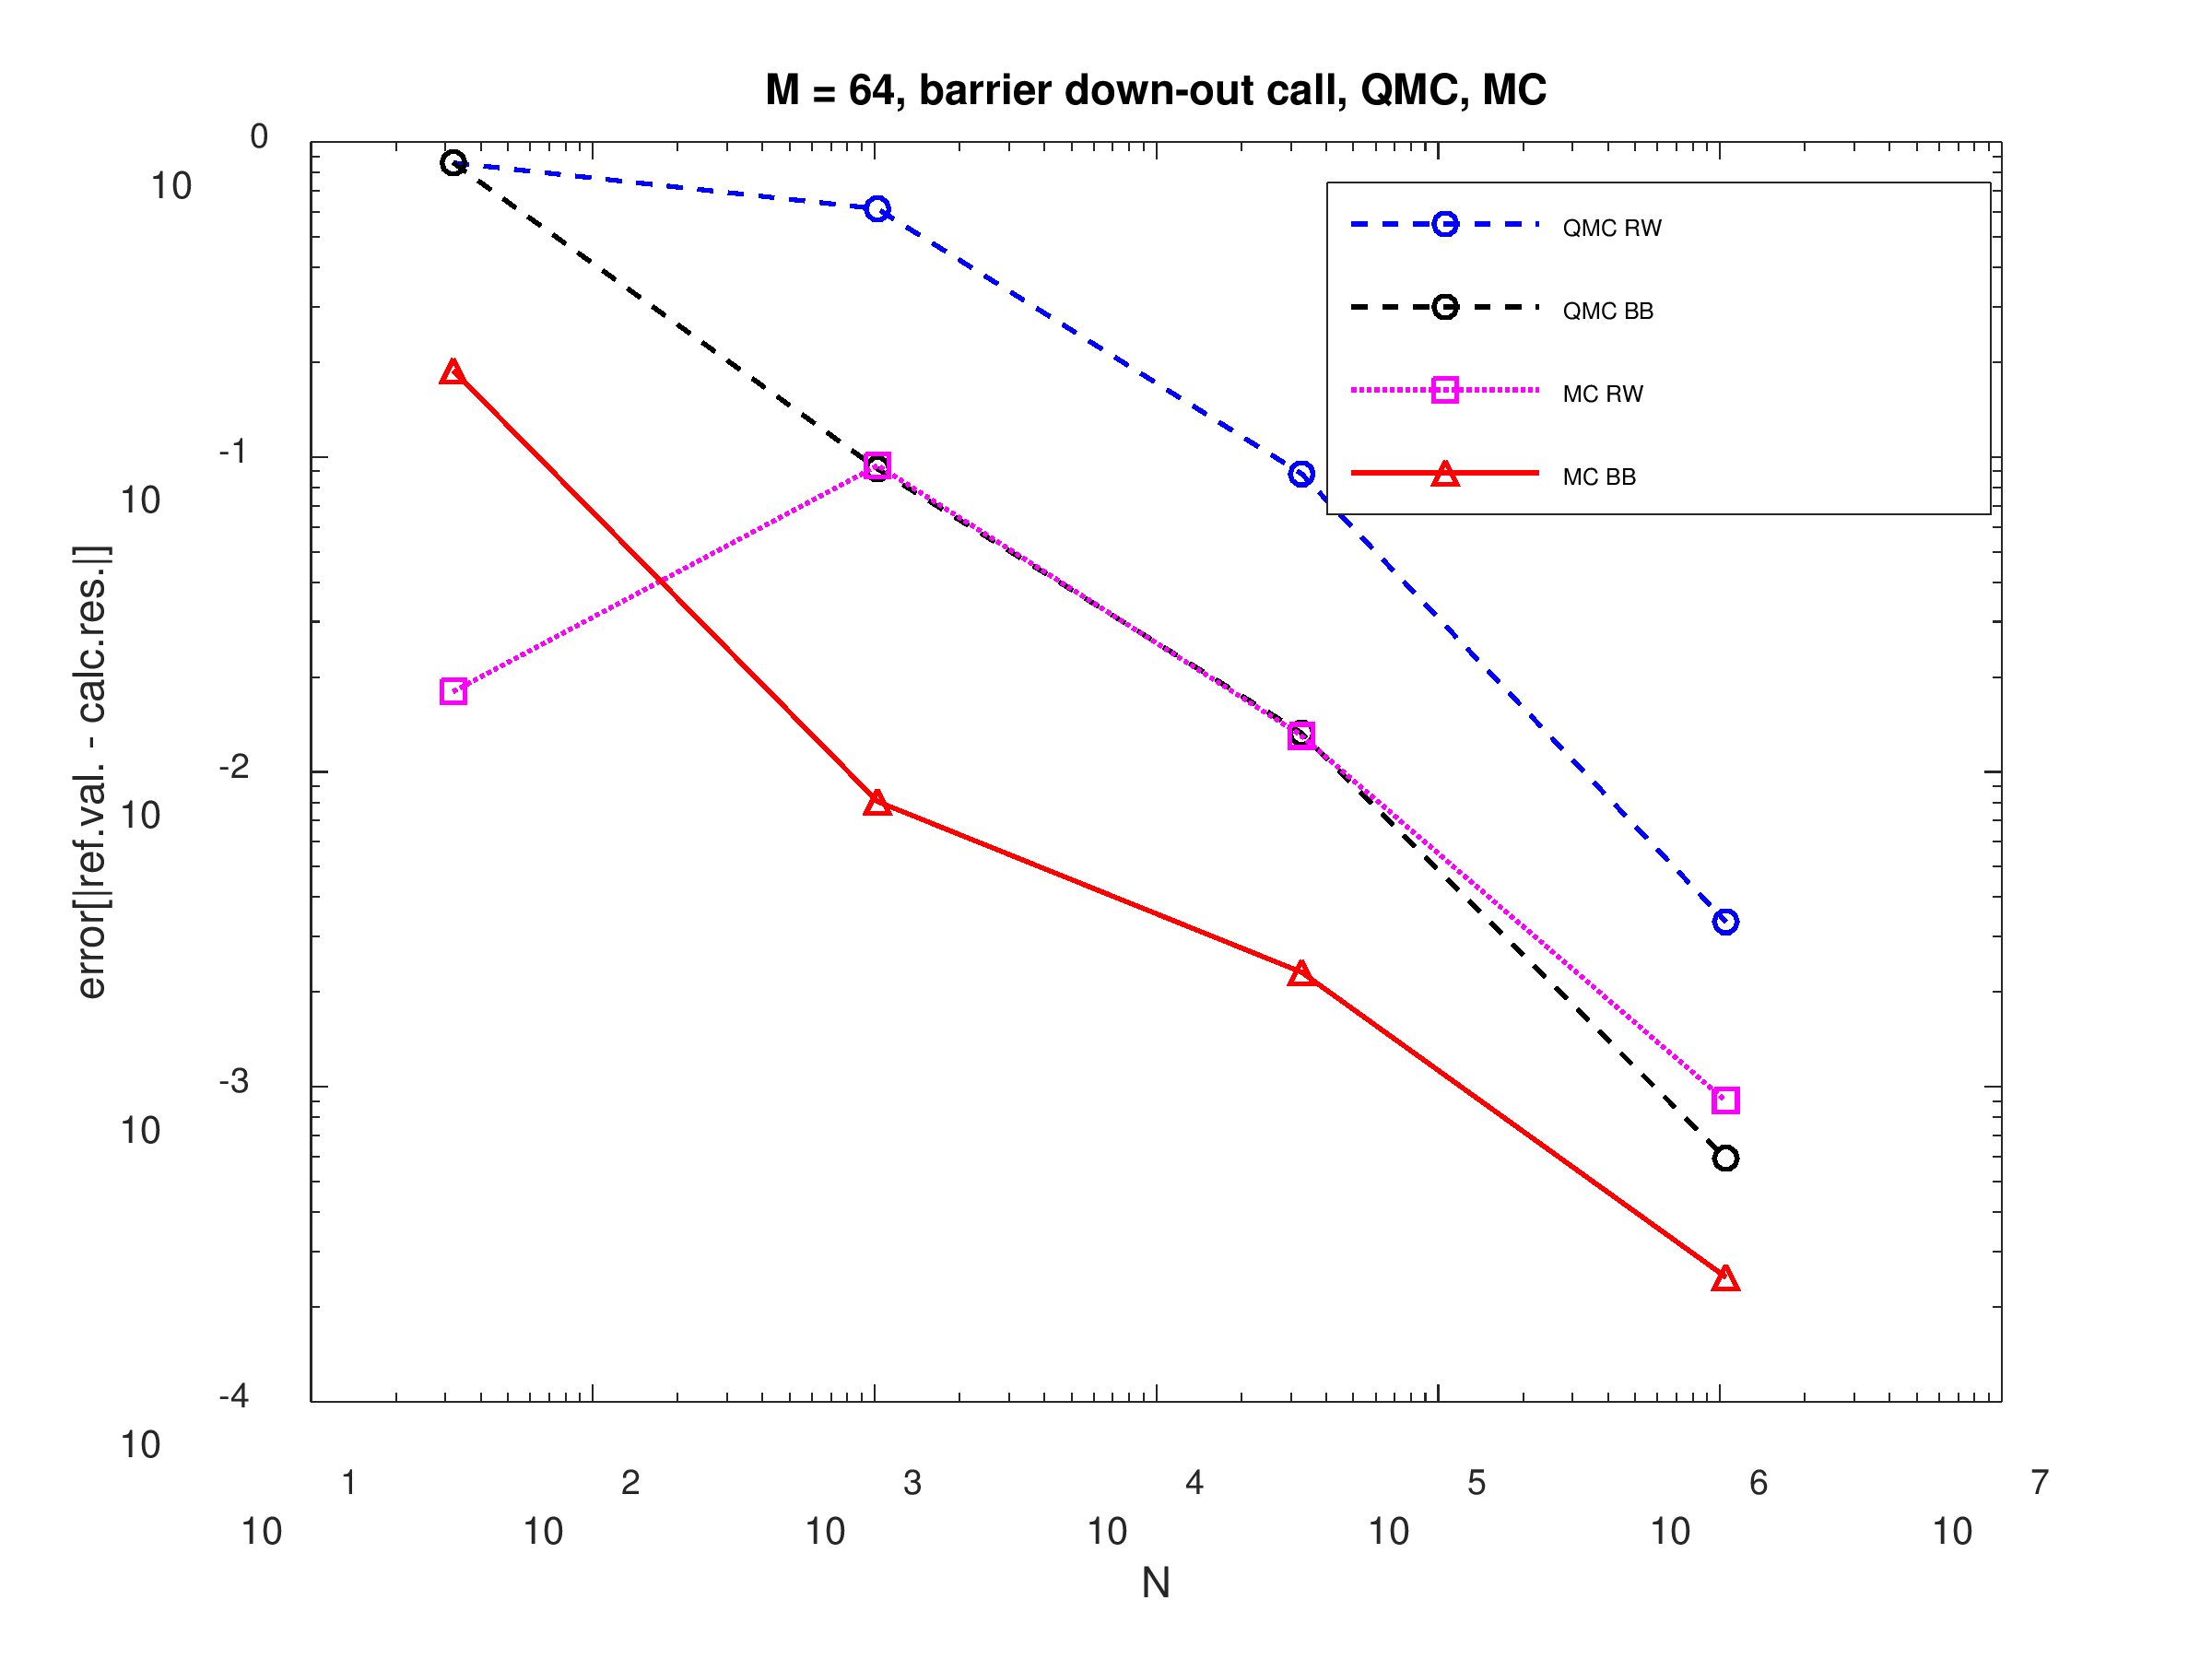
\includegraphics[scale=0.25]{images/task2_error.png}
\end{center}

\begin{itemize}
    \item{On this figure the absolute error: $|ref.val.-calc.val.|$ using different methods(QMC,MC) for Barrier Down-Out Call Option is plotted in loglog-scala against number of points.
    }
\item{
From the plots, one can observe that there is no really difference between using Brownian-Bridge or Random-Walk constructions.
}

\begin{center}
	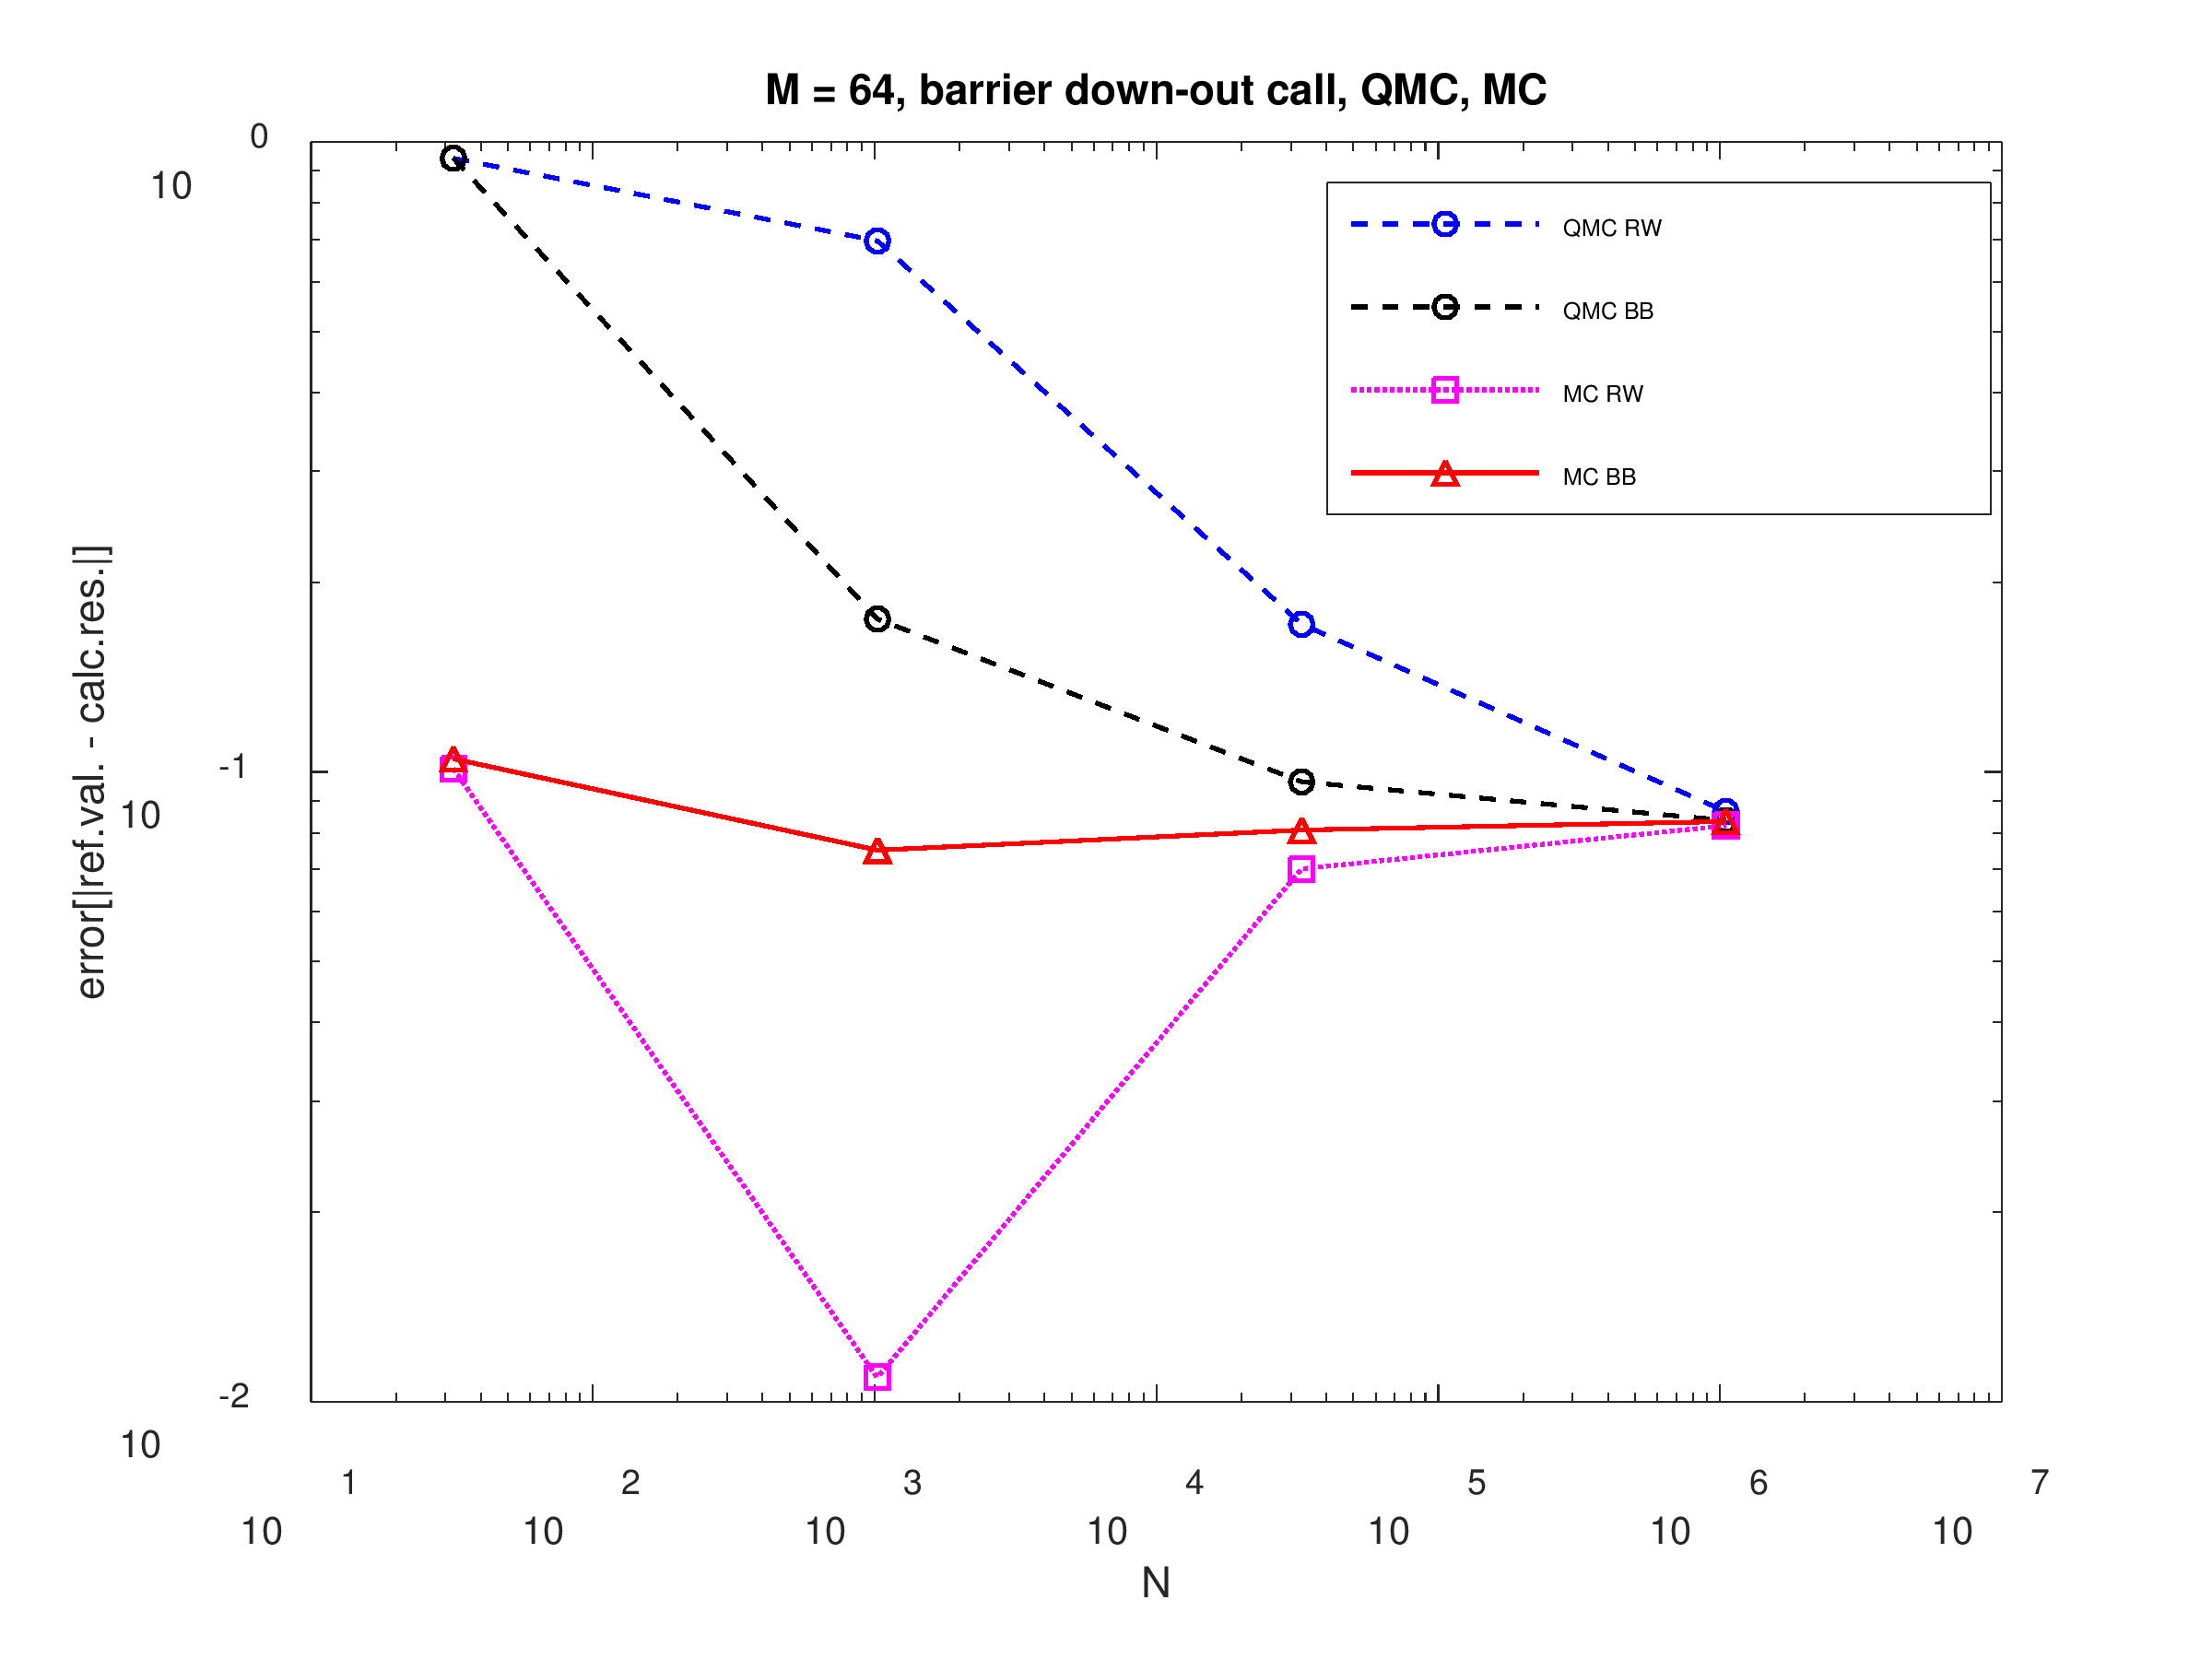
\includegraphics[scale=0.25]{images/task2_error_coarse_discretisation.png}
\end{center}
\item{
On this figure the absolute error: $|ref.val.-calc.val.|$ using different methods(QMC,MC) for Barrier Down-Out Call Option is plotted in loglog-scala against number of points. However now, reference value was computed using far more lower precision, where-from there is no convergence. 
}

\end{itemize}

\newpage

\section*{Task 3}

The picture below shows the fair price for a Down-Out call option with barrier $B$. One can see that the fair price is going down if the barrier is larger than about $B=8$. This makes sense, because when the barrier is high, the payoff is $0$ in many cases (because for this value of $B$ it happens more often that the price of the underlying is below the barrier).

\begin{center}
	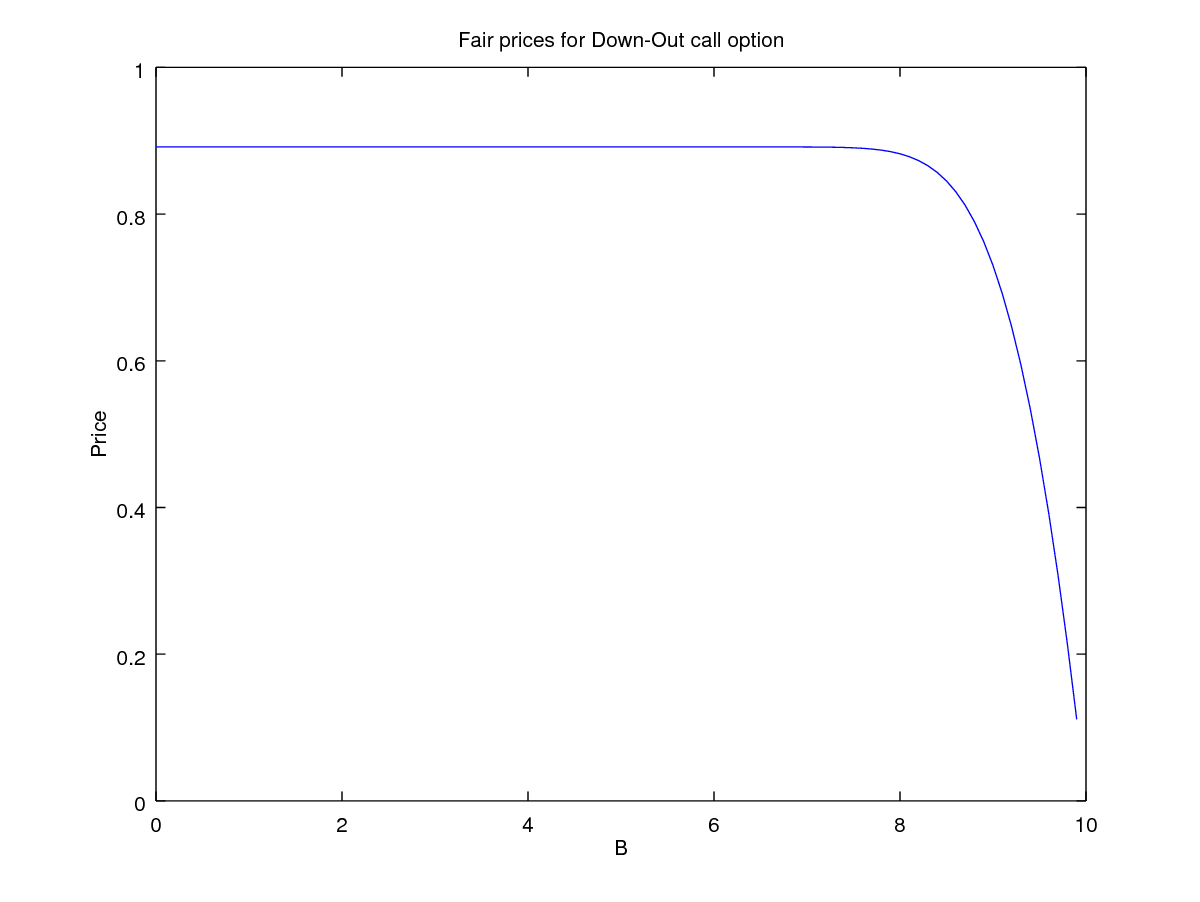
\includegraphics[scale=0.4]{images/fair_prices_down_out_call.png}
\end{center}

\section*{Task 4}
The next plot shows the absolute error for the discrete Down-Out call option for different values of $M$. One can see that for $M\geq64$ the convergence is much better than for $M=4$.  

\begin{center}
	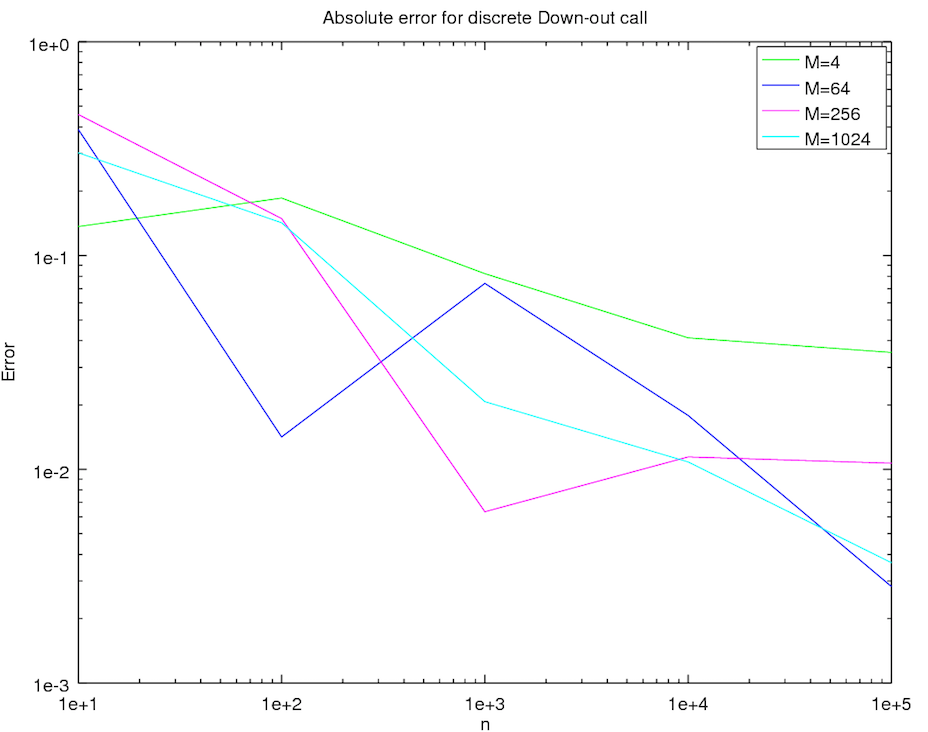
\includegraphics[scale=0.55]{images/convergence_plot_discrete_down_out_call.png}
\end{center}

\section*{Task 5}

\begin{center}
	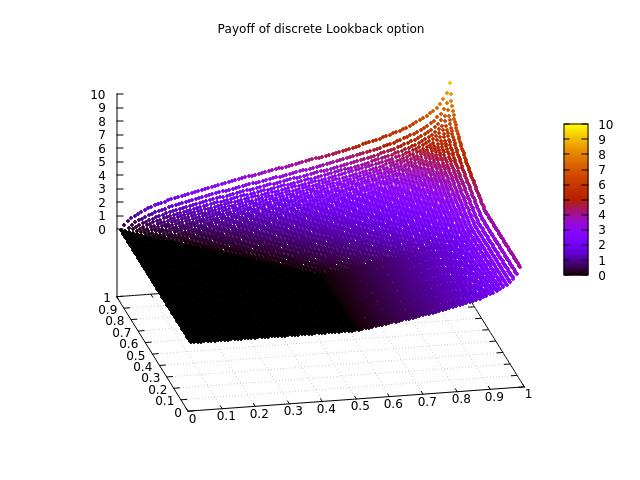
\includegraphics[scale=0.55]{images/payoff_lookback.png}
\end{center}

\section*{Task 6}

\begin{center}
	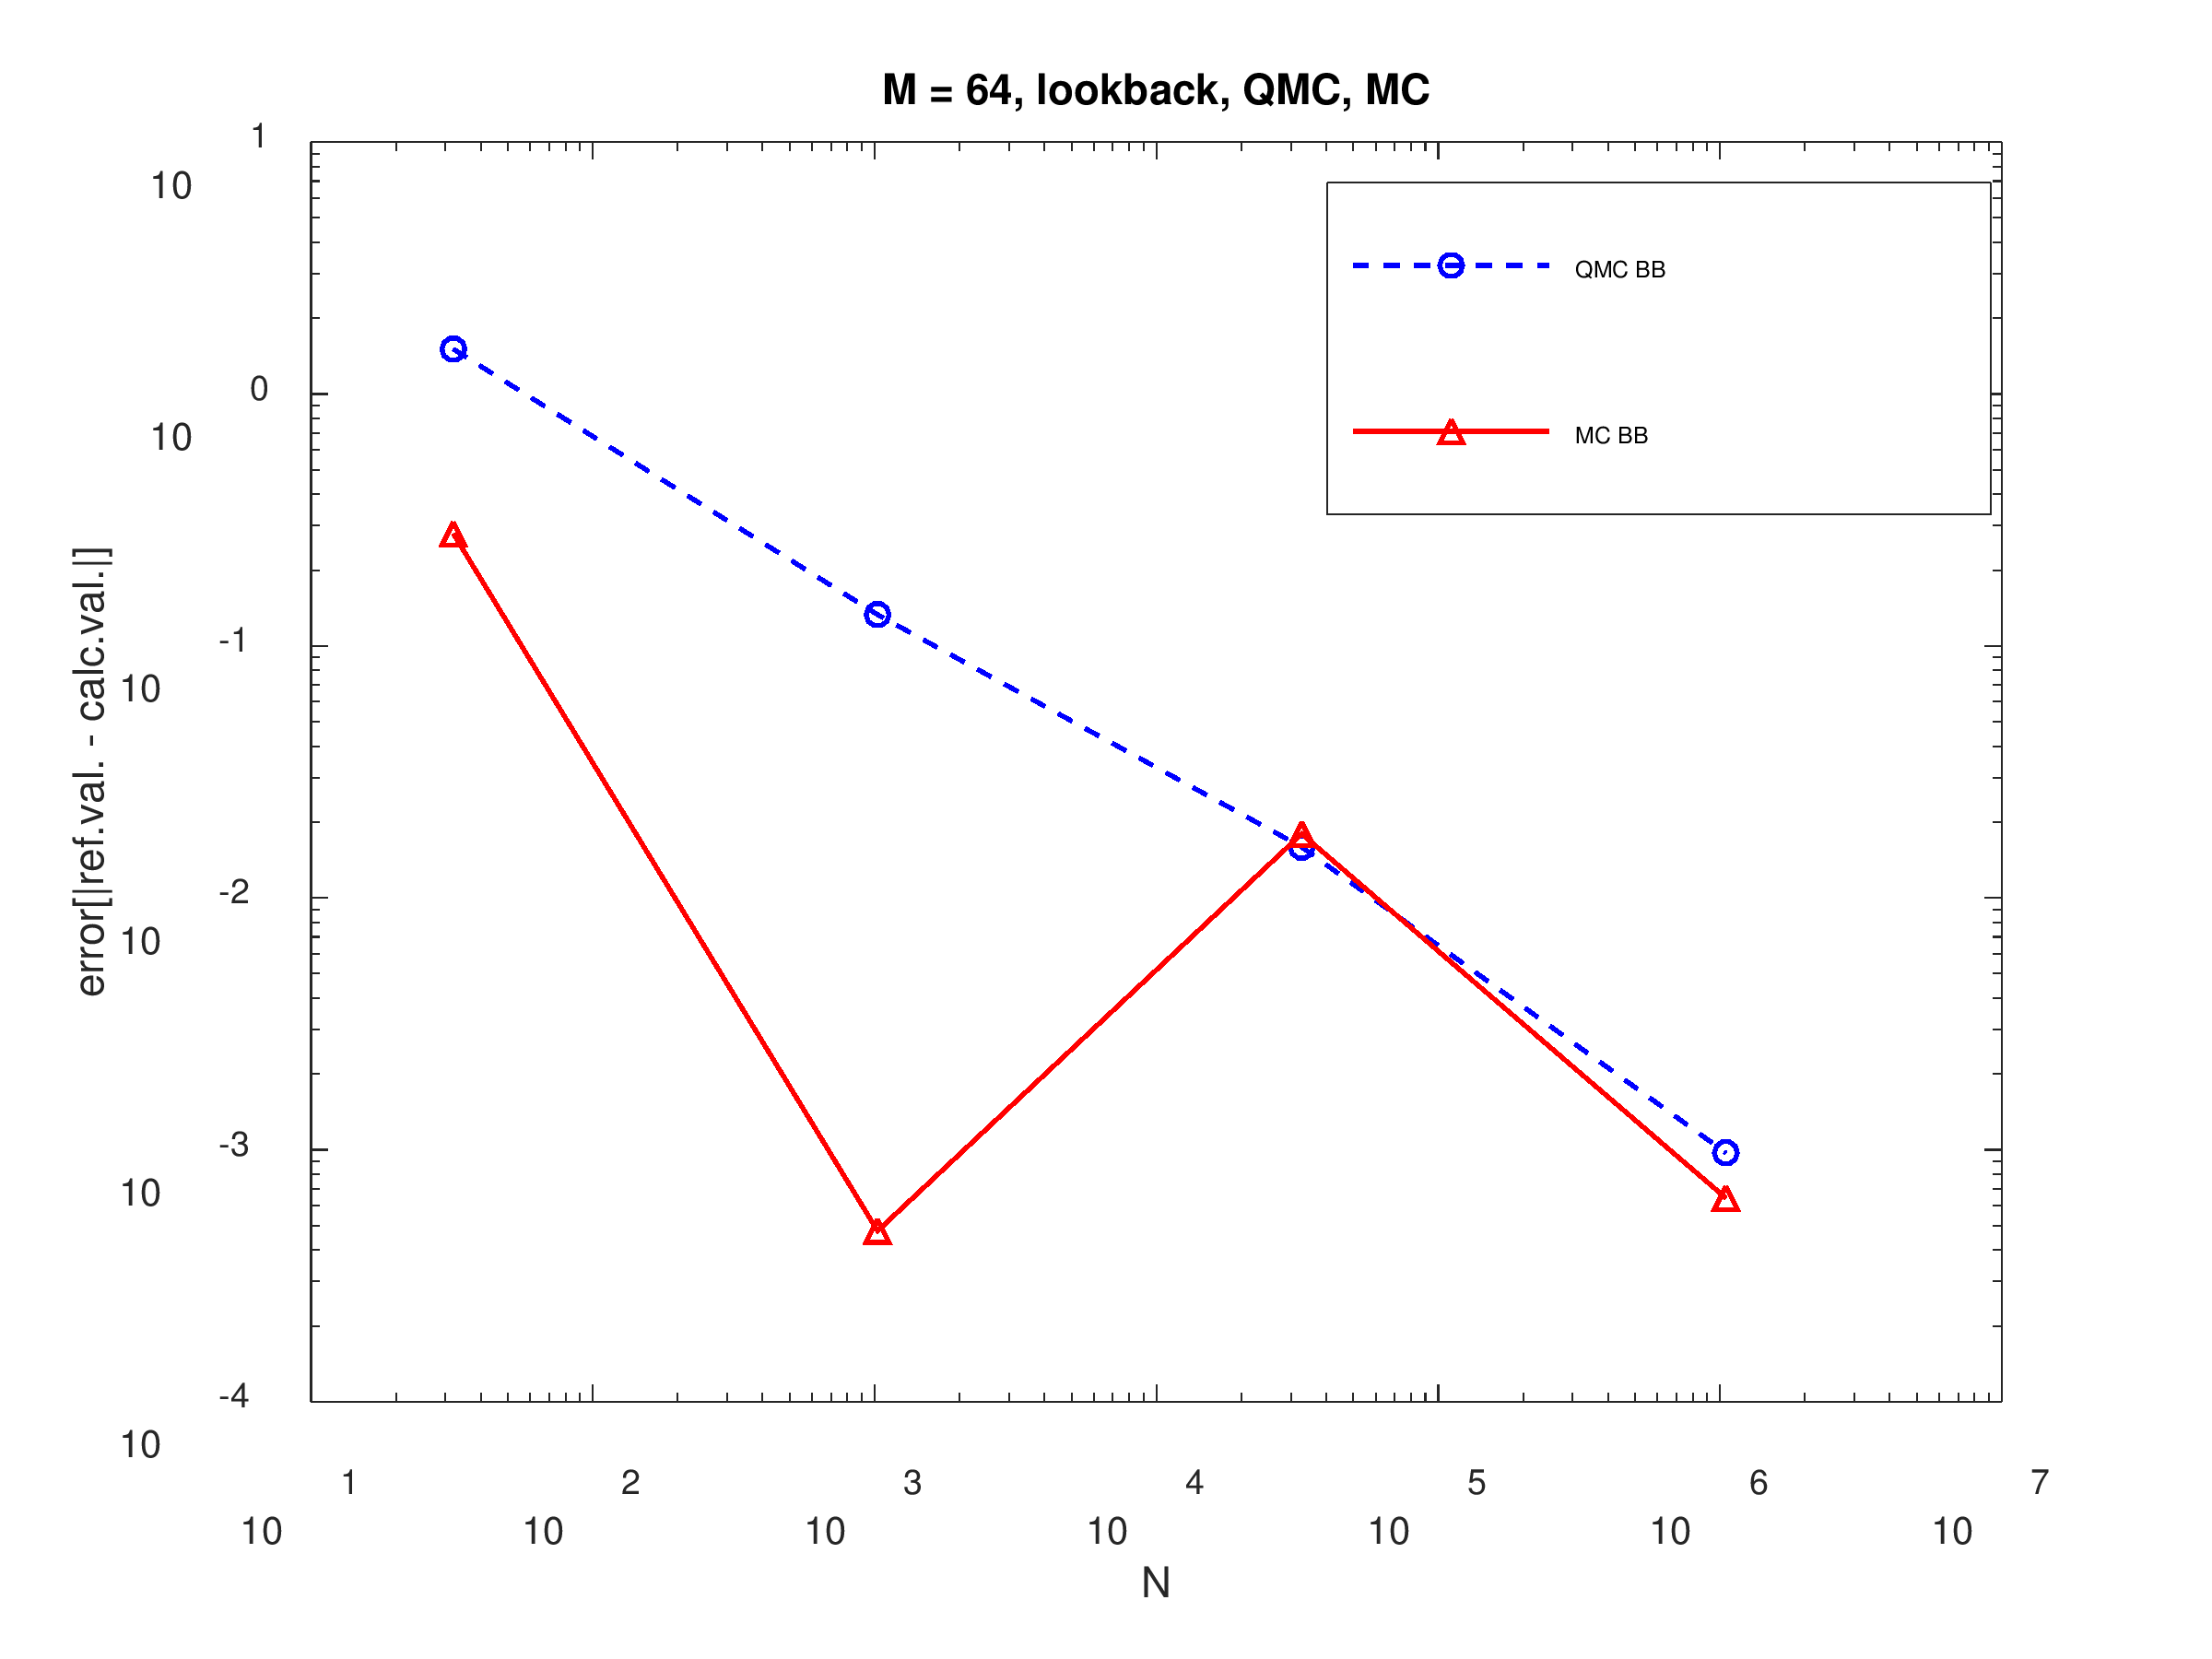
\includegraphics[scale=0.3]{images/task6_error.png}
\end{center}
\begin{itemize}
    \item{
        On this figure the absolute error: $|ref.val.-calc.val.|$ using different methods(QMC,MC with Brownian-Bridge) for Lookback Call Option is plotted in loglog-scala against number of points.
        
    }
     
\end{itemize}


\section*{Task 7}


\begin{center}
	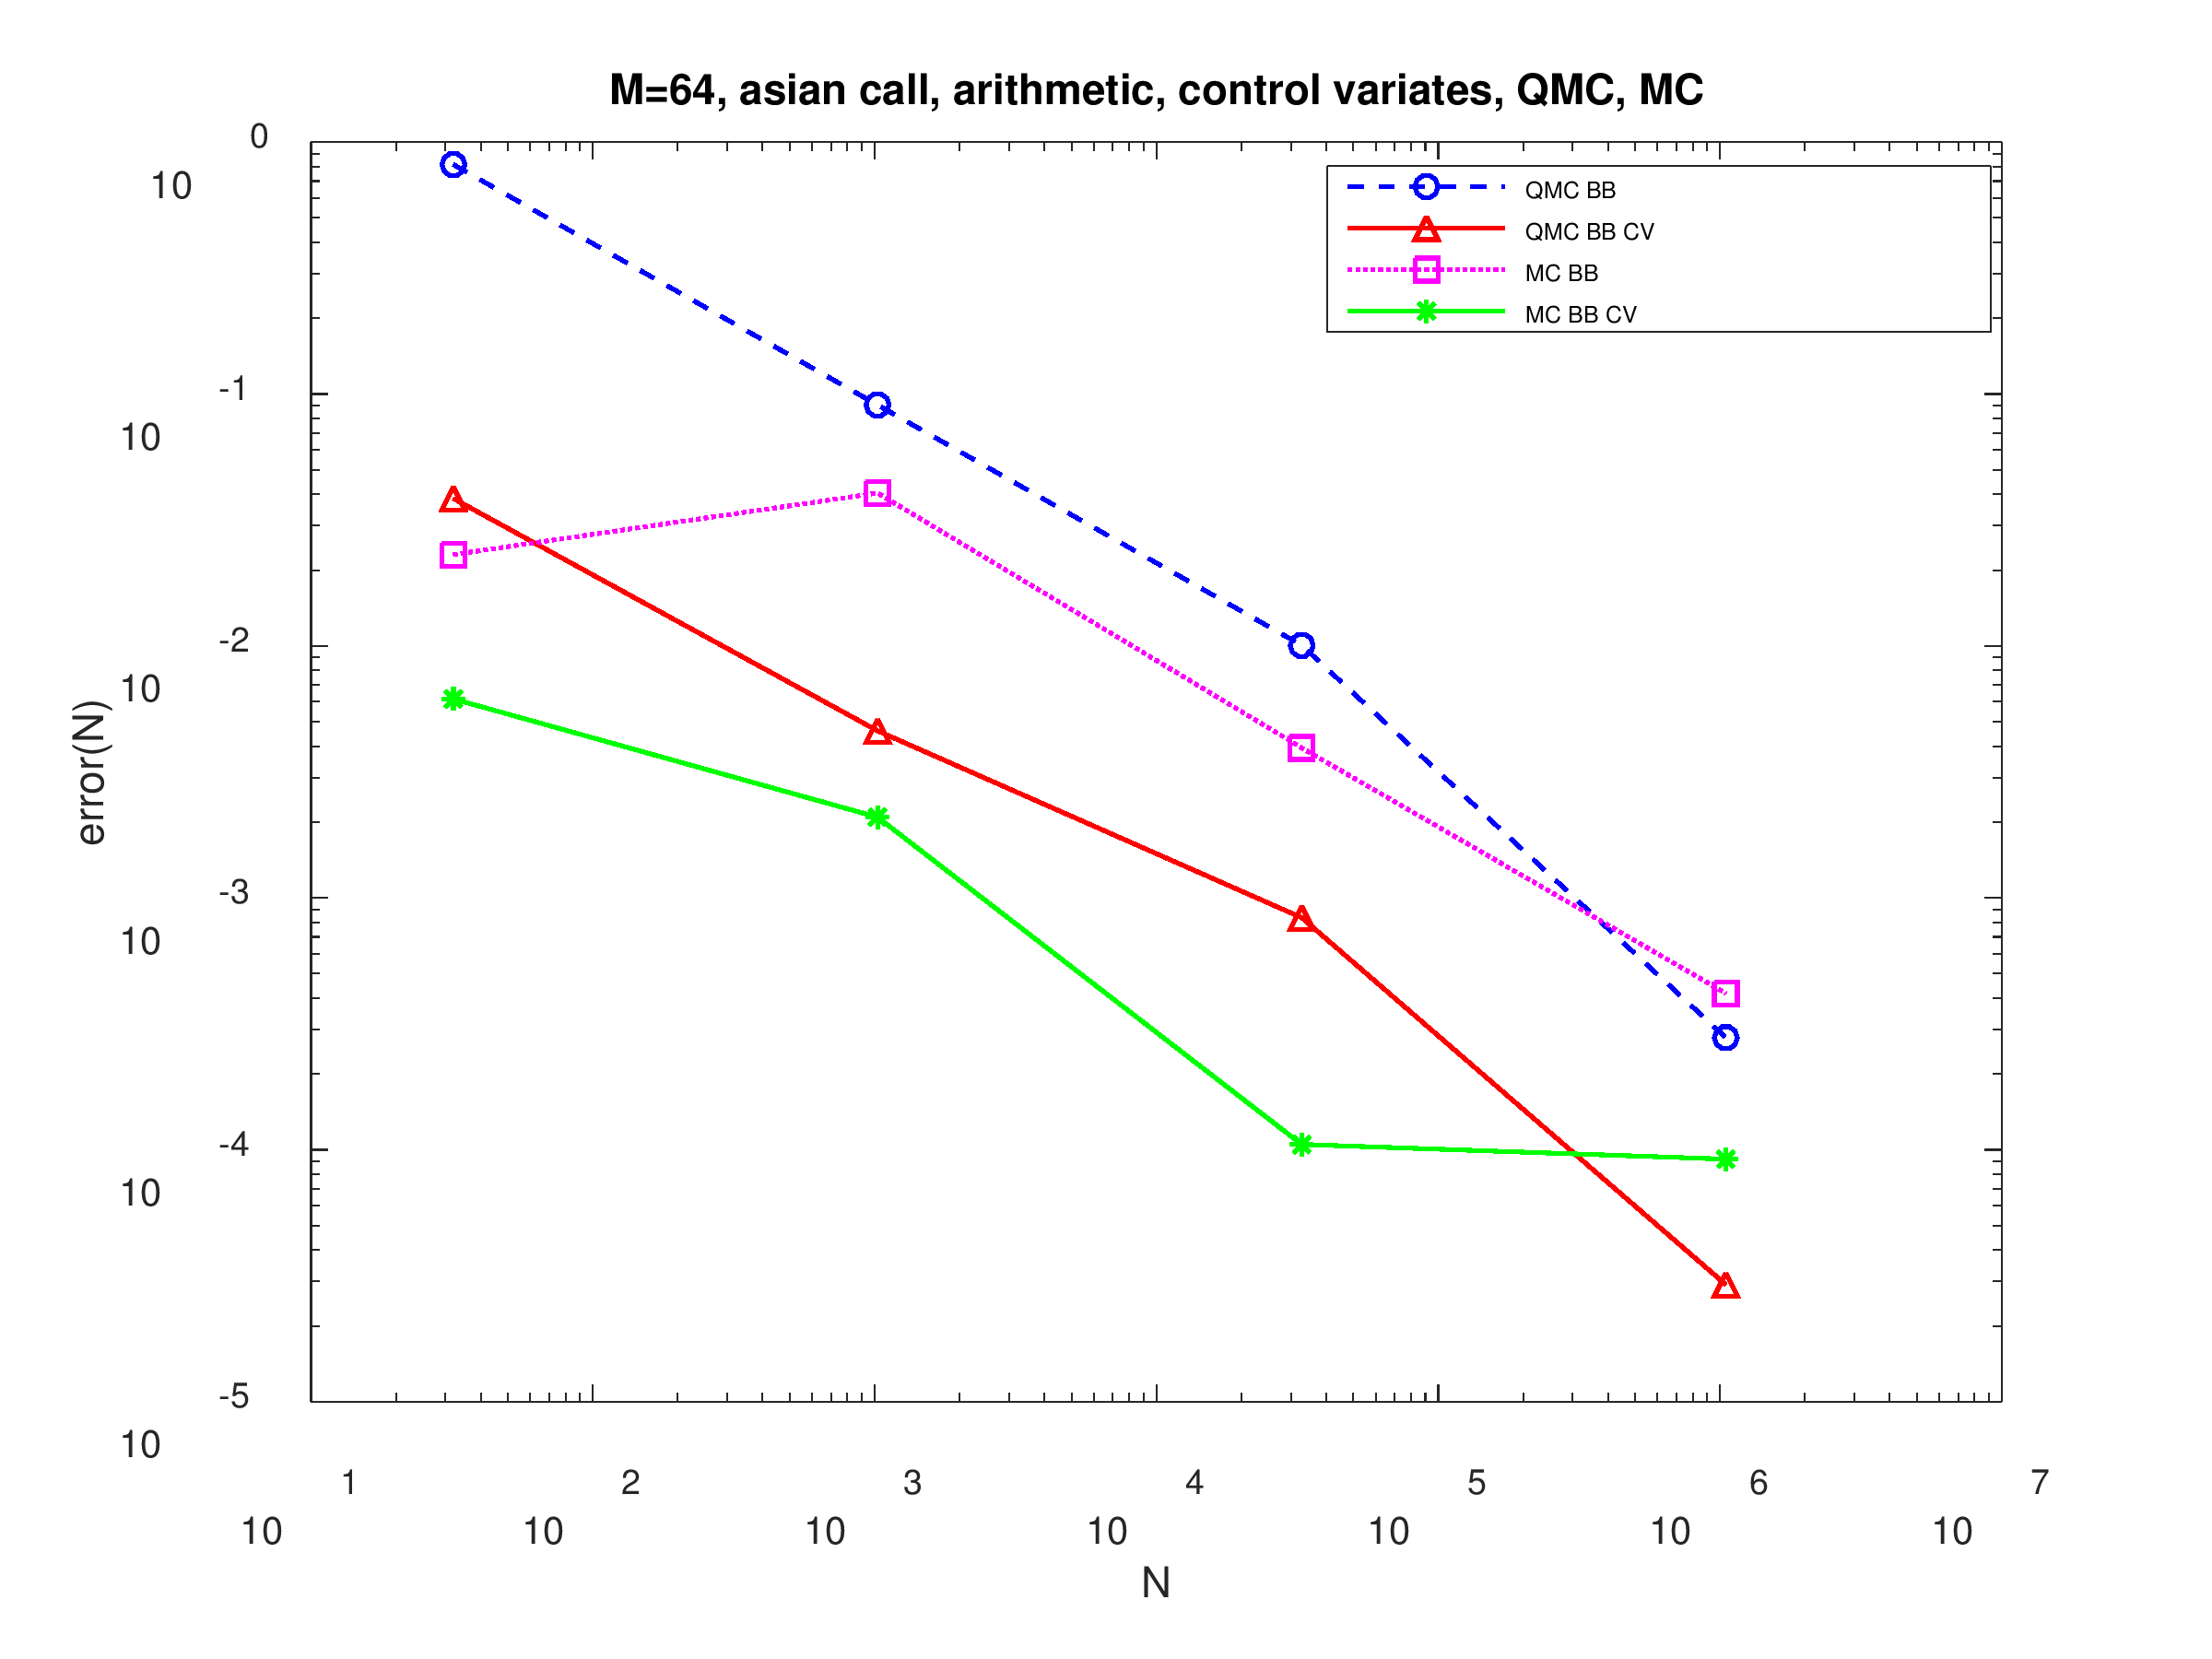
\includegraphics[scale=0.25]{images/task7_error.png}
\end{center}
\begin{itemize}
    \item{
        On this figure, results of the \textbf{control variate}
        method are presented. 
    }
\end{itemize}

\section*{Task 9}

\begin{center}
	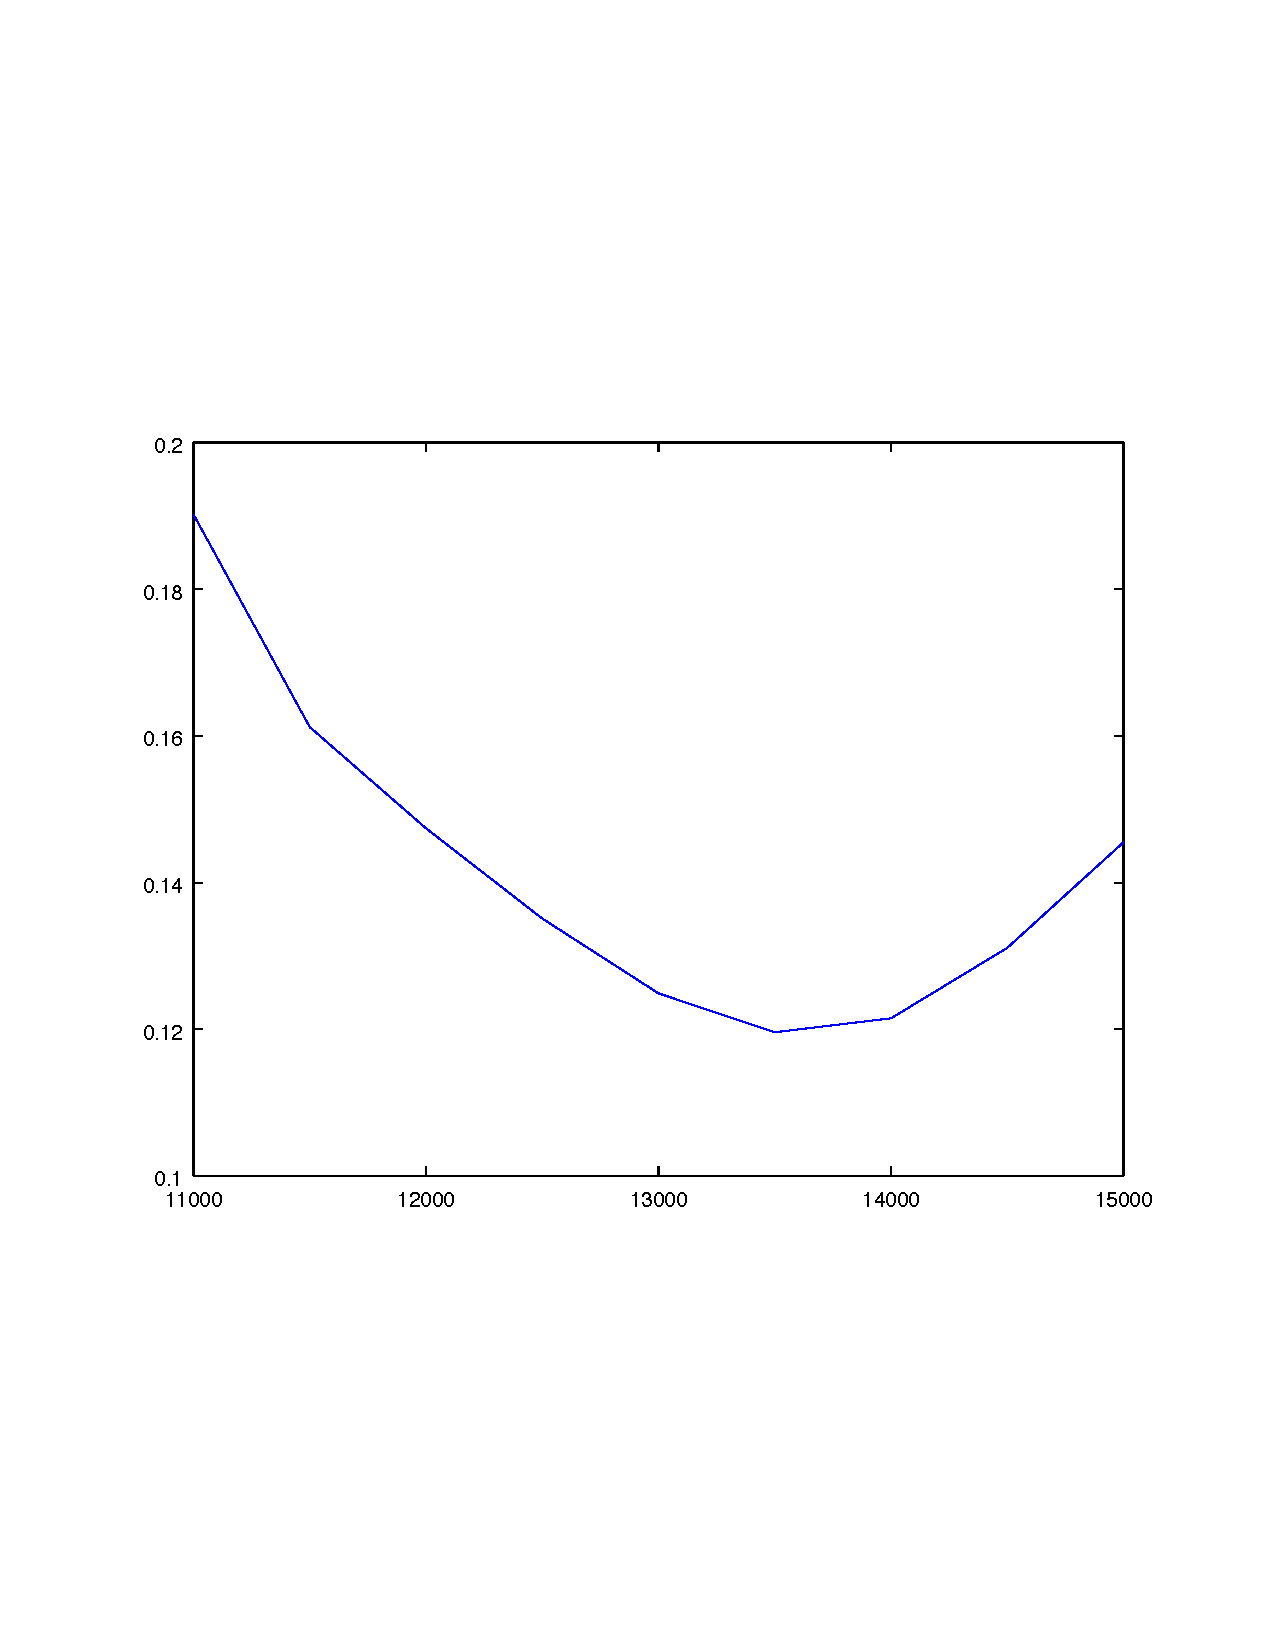
\includegraphics[scale=0.45]{images/dax.pdf}
\end{center}

Volatility of Call-Options for DAX, expiring in December, 2017. In this case, the volatility smile is clearly visible. The current value of the DAX is at about $12450$ points. 

\end{document}